% This is the root file of the thesis: thesis.tex

%%===================================
% \documentclass[12pt, oneside]{report}
\documentclass[12pt, twoside]{report}

\usepackage{url}
\usepackage[utf8]{inputenc} % This defines the font-encoding you prefer to use
\usepackage[pdftex]{graphicx}
\usepackage[bindingoffset=1cm,centering,includeheadfoot,margin=2cm]{geometry}

\usepackage[
    citestyle=numeric-comp,
    backend=bibtex,
    bibencoding=inputenc
    ]{biblatex}
\addbibresource{refs.bib}

\usepackage{setspace}
\linespread{1.5}
\setcounter{tocdepth}{2} 
\usepackage[colorlinks=true, pdfstartview=FitV,
linkcolor=blue, citecolor=blue, urlcolor=blue]{hyperref}
\setlength{\parindent}{0pt} % No indentation between paragraphs
\setlength{\parskip}{10pt} % Space between paragraphs

% Tables
\usepackage{ltxtable}
%\usepackage{arydshln}
%\usepackage{tabu, longtable}
\usepackage{booktabs}

% Needed for code listings
\usepackage{listings}
\usepackage{color}

% Subfigure
\usepackage{subcaption}

\usepackage{floatpag} % to move floatpagenr to topright

% Fussnote
\usepackage[hang]{footmisc}
\setlength{\footnotemargin}{-0.8em}

\usepackage{csquotes}
\usepackage{afterpage} % needed for empty page after front

%%===================================
% Custom definitions
    
% Signal color
\definecolor{signalColor}{RGB}{164, 63, 114}
\newcommand\signal[1]{\textbf{\textcolor{signalColor}{#1}}}
    
% List with less space between items
\newenvironment{cList}{
\begin{itemize}
  \setlength{\itemsep}{0pt}
  \setlength{\parskip}{0pt}
  \setlength{\parsep}{0pt}
}{\end{itemize}}

% Enumeration with less space between items
\newenvironment{cEnum}{
\begin{enumerate}
  \setlength{\itemsep}{0pt}
  \setlength{\parskip}{0pt}
  \setlength{\parsep}{0pt}
}{\end{enumerate}}

% Space LoL
\let\Chapter\chapter
\def\chapter{\addtocontents{lol}{\protect\addvspace{10pt}}\Chapter}

% Code definition JSON
\definecolor{numberColor}{RGB}{24,118,129}
\newcommand\JSONnumbervaluestyle{\color{numberColor}}
\newcommand\JSONstringvaluestyle{\color{signalColor}}

\newif\ifcolonfoundonthisline

\makeatletter

\lstdefinestyle{json}{
  showstringspaces    = false,
  keywords            = {false,true},
  alsoletter          = 0123456789.,
  morestring          = [s]{"}{"},
  stringstyle         = \ifcolonfoundonthisline\JSONstringvaluestyle\fi,
  MoreSelectCharTable =%
    \lst@DefSaveDef{`:}\colon@json{\processColon@json},
  basicstyle          = \ttfamily,
  keywordstyle        = \ttfamily\bfseries
}

\lstset{
  numbers=left,
  lineskip={-1.5pt},
  captionpos=b,
  basicstyle=\footnotesize\ttfamily,
  xleftmargin=1cm,
  breaklines=true
}

\newcommand\processColon@json{%
  \colon@json%
  \ifnum\lst@mode=\lst@Pmode%
    \global\colonfoundonthislinetrue%
  \fi
}

\lst@AddToHook{Output}{%
  \ifcolonfoundonthisline%
    \ifnum\lst@mode=\lst@Pmode%
      \def\lst@thestyle{\JSONnumbervaluestyle}%
    \fi
  \fi
  \lsthk@DetectKeywords% 
}

\lst@AddToHook{EOL}%
  {\global\colonfoundonthislinefalse}

\makeatother
% End code definition JSON

% Rename listings and toc
\renewcommand{\contentsname}{Table of Contents}
\renewcommand{\lstlistlistingname}{List of Listings}

\begin{document}

%%========================================
% Frontmatter

%!TEX root = ../thesis.tex

%This is the front page
%%=========================================
\thispagestyle{empty}


\includegraphics[width=\linewidth]{fig/Logo_Header}
\mbox{}\\[1pc]
\begin{center}
    \huge{ \bfseries Using Reinforcement Learning to Size Tasks for Scientific Workflows}\\[2pc]

    \Large{Nicolas Zunker}\\
    \large{n.zunker@campus.tu-berlin.de}\\[1pc]
    \large{December 13, 2021}\\[2pc]

    BACHELOR'S THESIS\\
    Distributed and Operating Systems Chair\\
    Technische Universität Berlin
\end{center}
\vfill

Examiner 1: Prof. Dr. Odej Kao
\hfill\llap{Advisor: Jonathan Bader}\\
Examiner 2: Prof. Dr. Volker Markl

\afterpage{\null\thispagestyle{empty}\newpage}
 % This is the titlepage
\setcounter{page}{0}
\pagenumbering{Roman}
%!TEX root = ../thesis.tex

%This is the Preface
%%=========================================
\cleardoublepage
\section*{Declaration}
\addcontentsline{toc}{section}{Declaration}
I hereby declare that I have created the present work independently and by my own without illicit assistance and only utilizing the listed sources and tools.\\

Hiermit erklaare ich, dass ich die vorliegende Arbeit selbststaandig und eigenhaandig sowie ohne unerlaubte fremde Hilfe und ausschliesslich unter Verwendung der aufgefaehrten Quellen und Hilfsmittel angefertigt habe.

Die selbständige und eigenständige Anfertigung versichert an Eides statt:
\begin{center}
Berlin, den 13. Dezember 2021\\[3pc]
Nicolas Zunker
\end{center}

%!TEX root = ../thesis.tex

%This is the Acknowledgment
%%=========================================
\cleardoublepage
\addcontentsline{toc}{section}{Acknowledgment}
\section*{Acknowledgment}

I would like to thank my advisor Jonathan for his helpful advice, constructive feedback and assistance, Prof. Dr. Toussaint, Prof. Dr. habil. Kao and Prof. Dr. Zubow whose courses I enjoyed immensely and from whom I learned a lot, and my friends and family for their support.

\nocite{fan2020,learningToSchedule,scarl,toussaint}


\begin{flushright}
NZ\\[1pc]
\end{flushright}

%!TEX root = ../thesis.tex

%This is the Summary
%%=========================================
\cleardoublepage
\addcontentsline{toc}{section}{Abstract}
\section*{Abstract}

The growth of computational power and the increasing importance of digital data in scientific research has led to greater demand for computational resources  by users who aim to process large datasets. Particularly in the natural sciences it has become common for scientists to break down their computing needs into a sequence of smaller tasks, a so called workflow. These workflows can then be run on a variety of different execution platforms, depending on the users needs.

Since workflows are composed of segregated inter-dependent tasks which can run independently of each other, the individual tasks which make up a workflow can be assigned a fraction of the computational resources available to the entire execution platform, and doing so intelligently could improve efficiency and performance.

This thesis aims to investigate how reinforcement learning can be applied to the allocation of resources to individual tasks in order to choose more efficient allocations. A reinforcement learning solution will be integrated into the source code of a popular scientific workflow management system and tested with several common bioinformatic workflows. Two different approaches (Gradient Bandits and Q-learning) will be used and their performance will be compared with both that of the default resource allocations and that of an approach based on \cite{tovarjob,FeedbackBasedAllocation} which uses a feedback loop.

Ultimately the approaches presented in this thesis outperform the workflow's default configurations with regards to both memory and CPU efficiency: the q-learning approach assigned 7\% less CPU hours, 31\% less memory and was 7\% faster, whereas the gradient bandit approach assigned 42\% less CPU hours, 80\% less memory and was only 4\% slower. The feedback loop approach assigned 13\% less CPU hours, 87\% less memory and was 7\% faster and thus performed worse than the gradient bandits with regards to CPU efficiency but better in terms of memory and speed. 

%%=========================================
%\cleardoublepage
\addcontentsline{toc}{section}{Zusammenfassung}
\section*{Zusammenfassung}

Die Relevanz von digitalen Daten und die damit verbundene Analyse von grossen Datensätzen in der wissenschaftlichen Forschung wächst kontinuierlich, und der Nutzerbedarf an Rechenressourcen steigt mit. Besonders in den Naturwissenschaften ist es üblich, dass Wissenschaftler die Analyse dieser Daten in kleinere Arbeitspakete aufteilen, so genannten Tasks, und die gesamte Sequenz dieser Tasks wird als Workflow bezeichnet. Die Workflows bestehen aus verschiedenen, eigenständigen Tasks die unabhängig voneinander ausgeführt werden können, daher muss ihnen nur ein Bruchteil der Rechenressourcen des Plattforms auf dem sie ausgeführt werden zugewiesen werden.  Durch intelligente Allokationen ermöglicht dies eine größere Effizienz und Leistung der Workflows.  

Die Forschungsfrage dieser Arbeit beinhaltet wie und mit welchem Effekt Reinforcement Learning für die Allokation von Rechenressourcen zu den Tasks eines Workflows angewandt werden kann.  Hierzu werden zwei verschiedene Ansätze (Q-learning und Gradient Bandits) in den Quellcode einer Workflow Verwaltungssoftware integriert und mit fünf Bioinformatik Workflows getestet. Diese Ergebnisse werden verglichen mit der Leistung der Workflows unter normalen Konfigurationen, und einem Ansatz mit Hilfe von Rückkopplungsschleifen, der auf \cite{tovarjob,FeedbackBasedAllocation} basiert.

Die in dieser Arbeit entwickelten Ansätze zeigten eine bessere Leistung als die Workflows mit voreingestellten Allokationen, sowohl im Bezug auf die Arbeitsspeichernutzung, als auch auf die CPU Nutzung.  Der q-learning Ansatz allozierte 7\% weniger CPU Stunden, 31\% weniger Arbeitsspeicher und die Rechenleistung war 7\% schneller. Der gradient bandit Ansatz allozierte 42\% weniger CPU Stunden, 80\% weniger Arbeitsspeicher und die Rechenleistung war nur 4\% langsamer. Letztlich hat der Ansatz mit der Rückkopplungsschleife 13\% weniger CPU Stunden und 87\% weniger Arbeitsspeicher alloziert und war 7\% schneller, und damit weniger effizient mit seiner CPU Allokationen als die gradient bandits aber besser in Bezug auf Arbeitsspeicher und Geschwindigkeit.

%\newpage
%\addcontentsline{toc}{section}{Zusammenfassung}
%\section*{Zusammenfassung}

%Der Aufstieg des Internet of Things (IoT) stellt uns vor neue Herausforderungen bezueglich der Speicherung, Verarbeitung und Darstellung von Daten

\tableofcontents

\clearpage
\phantomsection
\addcontentsline{toc}{section}{\listfigurename}
\listoffigures

\clearpage
\phantomsection
\addcontentsline{toc}{section}{\listtablename}
\listoftables

\clearpage
\phantomsection
\addcontentsline{toc}{section}{\lstlistlistingname}
\lstlistoflistings

%%=========================================
% Mainmatter

\cleardoublepage
\setcounter{page}{0}
\pagenumbering{arabic}
%!TEX root = ../thesis.tex

\cleardoublepage
\chapter{Deterministic Multipath Backhaul Exposee - Masters Thesis}

\label{cha:introduction}

%%=========================================
\section{Motivation and Problem Description}
\label{sec:motivation}

One of the aims for the fifth generation of mobile networks (5G) and it's successors will be a greater diversification of the classes of service. As the use cases for these networks evolve, there is a greater need for quality of service (QoS) tailored to each use case. For example, in Industrial Internet of Things (IIoT) applications the bandwidth requirements are often quite low, however the requirements on latency, jitter, and reliability may be extremely stringent. Supporting these kinds of classes of service can be a challenge for mobile network operators (MNOs) and will require novel approaches to familiar problems, such as backhaul.

With more backhaul solutions becoming available (i.e. LEO satellite links, and mmWave backhaul) and adding to the existing set of options (DSL, optical fibre, DOCSIS, dedicated lines, etc.) network operators may choose to utilize more than one backhaul connection at once in order to increase the available bandwidth or to utilize the different qualities of the backhaul links. Such a situation, could then be used to achieve higher quality of service by intelligently selecting on which link to forward packets. This approach bears similarity to multihoming as well as to multi-path routing, and can take inspiration from the existing body of research in these fields which has demonstrated that QoS can be improved by using multiple paths simultaneously \cite{akella2003measurement, tao2005improving, habib2007improving, goldenberg2004optimizing, huang2008multiconstrained, akella2008performance}.


%\LTXtable{\textwidth}{tab/scenario1_sensor}

%%=========================================
\section{Goal of the Thesis}
\label{sec:goal}

\begin{figure}[h]
    \centering
        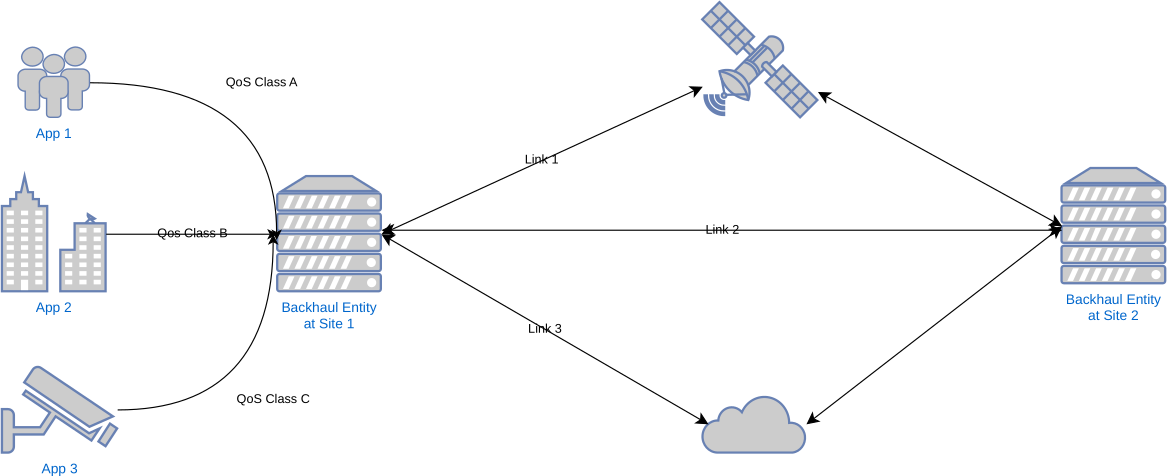
\includegraphics[width=\textwidth]{fig/use_cases.png}
        \caption{Use Case for the Backhaul Entity}
        \label{fig:use}
\end{figure}


\begin{figure}[h]
    \centering
        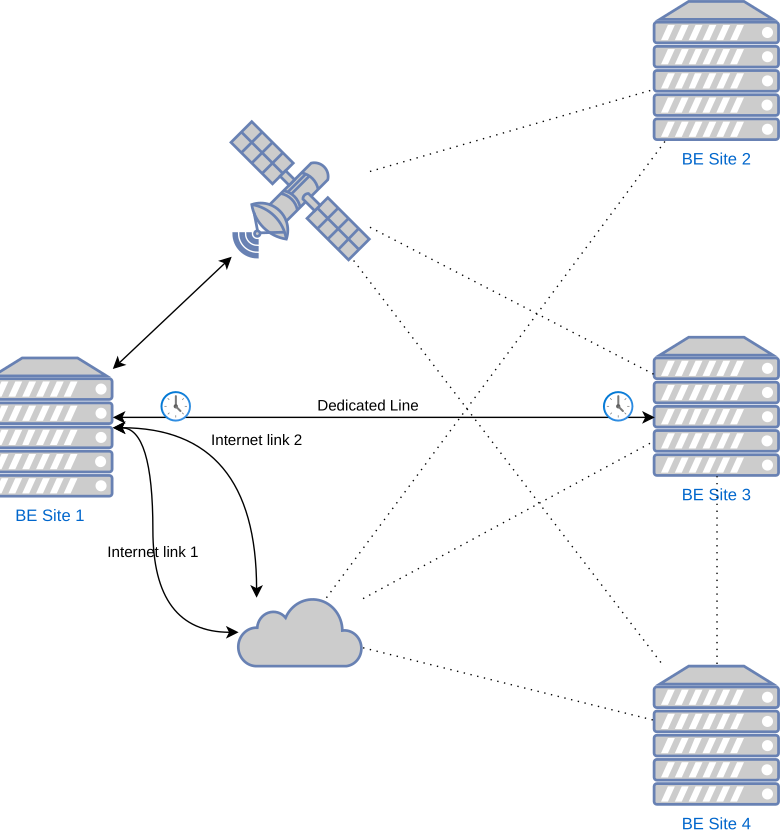
\includegraphics[width=0.75\textwidth, height=0.75\textwidth]{fig/mesh_network.png}
        \caption{Network of Backhaul Entities}
        \label{fig:mesh}
\end{figure}

The goal of this thesis is to design a backhaul entity, that can be placed at the ingress and egress point of connected networks, and which can intelligently forward packets on one or more links in order to meet specific QoS requirements. The performance of this approach will then be quantitatively analysed in experiments. Looking at figure \ref{fig:use} we can see how this is envisioned to work: A backhaul entity is deployed in 2 or more sites which have more than one egress link. Then, using the multiple links, the traffic is backhauled to the second site, while respecting it's QoS requirements. An example of how this entity could be deployed in multiple sites, interconnected in a mesh network, can be seen in figure \ref{fig:mesh}. This could allow network operators to provide more reliable quality of service for it's users, especially for important applications (e.g. between industrial sites).

%%=========================================
\section{Structure of the Thesis}
\label{sec:structure}

The planned work for the thesis will be structured as follows:

\begin{enumerate}
\item{\textit{Design}: Research existing approaches and solutions, and design an approach for reliable backhaul over multiple paths/links}
\item{\textit{Implementation}: Implement said approach in a basic testbed consisting of a traffic generator, various link emulators, measurement devices, and the backhaul entities}
\item{\textit{Evaluation}: Analyse the performance of the backhaul entity according to its ability to reduce latency, improve jitter, and provide any other QoS requirements. And compare it's performance with the performance of each individual link, as well as the performance of a round robin packet forwarding approach which utilises each link equally.}

\end{enumerate}

\begin{figure}[h]
    \centering
        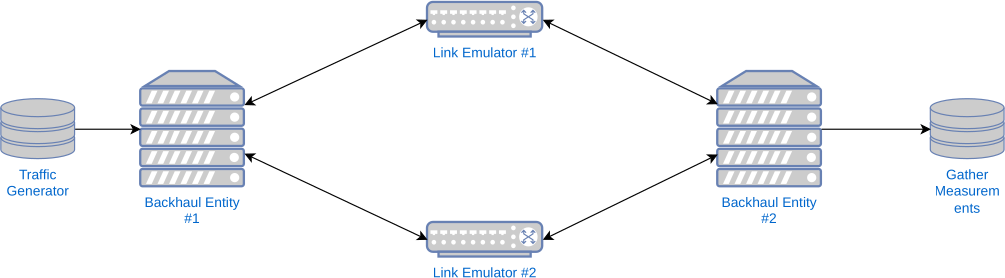
\includegraphics[width=\textwidth]{fig/testbed.png}
        \caption{Testbed Setup}
        \label{fig:testbed}
\end{figure}

The structure of the report will be a simple 5 chapter format: 1) Introduction, 2) Background and Related Work, 3) Approach, 4) Evaluation, 5) Conclusion. The approach chapter will discuss the proposed solution, and the evaluation chapter will encompass the design of the testbed and an analysis of the results.

\subsection{Timescale}

A thesis should take 6 months, or roughly 26 weeks. At present it is proposed to divide those 26 weeks into 4 equal sized chunks. The first 3 chunks will correspond to the 3 items mentioned previously in this section, the final "chunk" will be to finish writing up the report, however it is planned to do some writing during the other 3 chunks as well. In the first period - the \textit{Design} period, chapters 1 and 2 will also be worked on. After the \textit{Implementation} period is finished, chapter 3 can be written. Chapters 4 and 5 can then be written after the \textit{Evaluation} period finishes. That leaves the final chunk of time, which can be used to revise the document, as well as a buffer in case other parts of the thesis take longer to do.

The first phase of the experimental work will consist of setting up the testbed. This means installing the measurement modules as well as the link emulators. The next phase will require the implementation of the backhaul entity, as designed. The backhaul entity will require a module for collecting per-metric links, as well as the implementation of an algorithm to select the best link or links for a given flow. In the course of designing and preparing the backhaul entity there may be room for adjusting the initial plan based on what we experience during development. Next, the entity must be tested. During this phase traffic replays will be played over the testbed and evaluated. Thereafter the round robin approach and the "god routing" approach will also be evaluated. These two approaches will serve for comparison with the performance of the backhaul entity. Finally, this data must be analyzed, and the thesis can reach its conclusions, with 1 or 2 weeks buffer room for last minute revisions.


\begin{figure}
\begin{ganttchart}[expand chart=\textwidth, vgrid, hgrid]{1}{26}
  \gantttitle{Week}{26} \\
  \gantttitlelist{1,...,26}{1} \\
%  \ganttgroup{Group 1}{1}{7} \\
  \ganttbar{Literature Review}{1}{2}  \ganttbar[bar/.append style={fill=lightgray}]{}{3}{4} \\
  \ganttbar{Setup Testbed}{2}{4} \\
  \ganttbar{Implement Approach}{4}{8}] \ganttbar[bar/.append style={fill=lightgray}]{}{9}{10}  \\
  %ganttbar[bar/.append style={fill=lightgray}]{}{14}{14} \\
  \ganttbar{Metric Collection}{5}{7} \\
  \ganttbar{Link Switching Algorithm}{6}{8}\\
  \ganttbar{Adjust and Improve}{7}{9} \\
  \ganttbar{Measurements}{10}{16}  \ganttbar[bar/.append style={fill=lightgray}]{}{16}{18} \\
  \ganttbar{Round Robin}{12}{14} \\
  \ganttbar{God Routing}{14}{16}  \\
  \ganttbar{Evaluation}{18}{20}  \ganttbar[bar/.append style={fill=lightgray}]{}{21}{22} \\
  \ganttbar{Finish Writing Thesis}{21}{23}  \ganttbar[bar/.append style={fill=lightgray}]{}{24}{26} \\
  % \ganttlinkedbar{Task 2}{3}{7} \ganttnewline
 % \ganttmilestone{Milestone}{7} \ganttnewline
  \ganttlink{elem2}{elem3}
  \ganttlink{elem4}{elem8}
  \ganttlink{elem5}{elem8}  
  \ganttlink{elem6}{elem8}
  \ganttlink{elem7}{elem8}

 \ganttlink{elem9}{elem12}
 \ganttlink{elem10}{elem12}
 \ganttlink{elem11}{elem12}

\ganttlink{elem12}{elem14}

\end{ganttchart}
\caption{Gantt Chart: 01.06.23 - 01.12.23}
\end{figure}

\section{Envisioned Approach}

\subsection{Collecting Per-Link Metrics}

In order to realize such a backhaul entity, the entity needs to be able to maintain a set of metrics about the available links to aid it in choosing which links to utilize. This may not always be straightforward, and could require prediction of link quality based on previous measurements.

\subsubsection{Measurement-based Metrics}

In \cite{akella2008performance} the authors collected both passive metrics (looking at response times for outgoing packets), and active measurements (sending ICMP ping, or TCP SYN messages and measuring the response time). It is important to note that using the passive measurements enabled their multihomed approach to perform well, but when using the active measurements the performance was better. Crucially, the passive measurements worked better over larger sampling periods because it took longer to get a full overview of all the possible routes. Whereas the active sampling approach acquired it's measurements faster and was thus more effective over smaller sampling intervals.

Considering these results, it is proposed to utilize both active and passive measurements. All three metrics- packet loss, latency, and jitter- will be periodically measured in an active manner, on a site to site basis. The period over which to perform these measurements is an important design decision.

Beyond this, these metrics will also be monitored on a passive basis wherever possible. For all three metrics a response is required for each sent message, in order to measure either the time needed (for latency and jitter), or to ascertain a packet has been lost. This may only be possible for TCP SYN and SYN ACK messages, and other protocols which are guaranteed to contain certain request-response handshakes.

\subsection{Pre-configured Metrics}

Since certain links may be come with hard guarantees on packet loss, latency and jitter, this would drastically simplify the process, and thus allow us to save ourselves the measurement process for said links. Therefore the backhaul entity which will be designed, shall allow for a link to have the jitter, reliability and latency metrics pre-configured, as well as allowing them to be updated while the entity is running.

\subsection{How to Guarantee QoS}

The design of this approach is also an interesting challenge. One idea to improve jitter when backhauling across multiple links is to duplicate packets and forward them on multiple links, and have the backhaul entity on the other end buffer incoming packets and release them at a constant rate. This way in the event of a packet being lost on one link, the other link is still able to receive it and the delay caused by retransmission is avoided. The downside with this approach is that it guarantees the latency will always be that of the slowest link.

For reducing latency it would appear likely that the simplest approach may be a greedy method (as in \cite{goldenberg2004optimizing} in the online case) which always selects the lowest latency connection. However there is room for nuance here since the connection must not be overloaded and also because certain traffic may have very relaxed latency requirements but use up more bandwidth. This means monitoring the load on any one link will be important. Finally there are also more intelligent approaches, i.e. integer linear programming (used in \cite{huang2008multiconstrained} and for the offline case in \cite{goldenberg2004optimizing}) which could be used to optimally satisfy certain requirements.

The timescale over which to use a chosen link is also of interest. In \cite{habib2007improving} the time for which a link should be used is varied based on the predicted qualities of the link. These predictions are made based on past performance.

Reliability presents yet another challenge, however in a multihomed scenario it becomes easier to guarantee this via duplication, and/or forward error correction (FEC). For example if a packet flow requires 99\% reliability this can be guaranteed by duplicating packets across two links which are both only 90\% reliable. Alternatively, in such a situation, FEC could be used to pre-code the packets in order to provide the additional guarantees against packet loss and thus increase the reliability to the required level.

\subsubsection{Proposed Solution}

The solution proposed for solving this multi-constrained QoS problem is to use integer linear programming (ILP). Although ILP is NP-Complete, we can parameterize the problem by the number of outgoing links, which never needs to be more than 4, and thus brute force the solutions. The ILP constrained problem will be to select those links on which to forward packets while minimizing the overall number of links used, and making sure to satisfy the latency, jitter and reliability requirements of the given flow.

\begin{gather}
\text{Minimize } \sum_{i=1}^{P}x_i \\
\text{Where, } d(i) * x_i\le D \\
j(i) * x_i \le J \\
\text{and }1 - \prod_{i=1}^{P}{ ( 1- r(i) * x_i ) } \ge R  \\
\text{for } x_i \in \{0,1\}
\end{gather}

Here the variables $D$, $J$, and $R$ are the flow's delay, jitter, and reliability requirements, while the functions $d(i)$, $j(i)$, $r(i)$ are the predicted delay, jitter, and reliability of the link $i$ out of the $P$ total links. The predicted values will usually just be the latest measurement, as recommended in \cite{akella2008performance}, however there is room here to use more advanced metrics to predict the future link quality and thus perform preemptive path switching. The $x_i$ variable indicates whether or not link $i$ shall be used. If a solution is found, then the flow's packets will be forwarded on each link $i$ where $x_i = 1$, and if no solution can be found which satisfies these conditions then the flow is rejected because its QoS cannot be guaranteed.

\subsection{Potential Issues and Design Questions which are Still Open}

At present the idea would be to use the GTP protocol to tunnel data between any two backhaul entities, and then use the tunnel endpoint IDs (TEIDs) to differentiate between different traffic flows. In the control plane of the backhaul entity, one link would be chosen to be used for control and co-ordination messages between the two backhaul entities.

This approach could run into trouble if there is fragmentation. Some applications attempt to base their packet sizes on the most common MTU values for ethernet links (1500 bytes  minus 20 bytes for the IPv4 header and 2 bytes for UDP), and this causes a problem when the packet is tunneled because the overhead of another IP header on top of the tunnel header pushes the packet beyond the MTU and thus it has to be fragmented, which can degrade performance. In the proposed design of the testbed, there is a traffic generator at use, so this generator can be configured not to  generate packets exceeding 1450 bytes, but this issue is of practical concern for any realistic deployments.

\subsection{Evaluating Performance}

In order to evaluate the success of the proposed approach, three scenarios will be set up and investigated. Each setup will consist of two backhaul entities, and some number of emulated links going between them. The first scenario will feature 2 WAN links, a dedicated line, and a satellite connection. The second scenario will not feature the dedicated line, since it is expected that a leased line may be too obvious a choice for any of the traffic with strict QoS requirements. Finally, in order to further investigate these situations with an obviously superior candidate, the third scenario will just feature two links, a dedicated line and a WAN link.

In all of these scenarios the same traffic flows will be replayed. This traffic will contain various types of flows, with various QoS requirements. Before a new flow is started, the flow's requirements are sent to the backhaul entity and it is either accepted or rejected. During the traffic replay, the delay, jitter, and reliability will be measured.

These measurements will be performed once with the ILP approach proposed earlier and once with a simple round-robin approach for selecting links, and finally compared against an offline approach, where the optimal decision is computed with complete knowledge of the future. This offline approach will serve as the baseline for optimal performance, against which the other two approaches can be compared.


%%% include all citations

% start zotero

%\nocite{kundel_user_2022}
%\nocite{goldenberg_optimizing_nodate}
%\nocite{lange_performance_2015}
%\nocite{tarique_survey_2009}
%\nocite{tschoke_time-sensitive_2021}
%\nocite{ganichev_yamr_2010}
%\nocite{habib_improving_2007}
%\nocite{tao2005improving}
%\nocite{fanglu_guo_experiences_2004}
%\nocite{akella_measurement-based_nodate}
%\nocite{noauthor_zotero_nodate}

% end zotero...

% google translate

\nocite{tsai2006review}
\nocite{tao2005improving}
\nocite{kundel2022user}
\nocite{goldenberg2004optimizing}
\nocite{lange2015performance}
\nocite{tarique2009survey}
\nocite{tschoke2021time}
\nocite{ganichev2010yamr}
\nocite{habib2007improving}
\nocite{guo2004experiences}
\nocite{akella2003measurement}
\nocite{ergencc2021reliability}
\nocite{tao2004application}
\nocite{alwan2010multi}
\nocite{prados2021asynchronous}
\nocite{zhang2016fundamentals}
\nocite{chen2020collaborative}
\nocite{akella2008performance}
\nocite{andreoli2017mobile}
\nocite{huang2008multiconstrained}



%!TEX root = ../thesis.tex

\cleardoublepage
\chapter{Background}
\label{cha:background}


This chapter provides background information and explanations of the functionality and purpose of some of the technologies and concepts related to this thesis.  To begin the history of cloud computing and containerization are discussed in sections \ref{sec:cloud} and \ref{sec:containers} before moving on to a discussion of their current usage in scientific workflows in \ref{sec:workflows}. After that, the target software, nextflow, of this thesis is introduced in section \ref{sec:nextflow}. Finally, in \ref{sec:rl} reinforcement learning is touched upon and the benefits it could bring to the problem at hand are briefly explained.

%%=========================================
\section{Cloud Computing}
\label{sec:cloud}

The principle behind computer clusters is to pool the resources of several machines to speed up the execution of a program as well as to leverage specific data and or hardware resources of other machines in the cluster. This has given rise to the concept of cloud computing which takes this principle and aims to make these clusters of machines more accessible and configurable. Cloud computing aims to be available all the time and from anywhere, and to provide configurable computing resources to support the needs of the user. The most common resources in demand are data storage and computational power. With the rise of the internet and the increasing demand for  computational power, cloud computing continues to grow in popularity. 

%%=========================================
\section{Containerization}
\label{sec:containers}

Virtualization has existed for a long time however the overhead of running a virtual machine is often not worth the advantages they provide. Particularly for reproducible software development the most important qualities of the host machine beyond the architecture are the operating system and its filesystem. Since most applications these days need to run on multiple servers and it these can quickly become difficult to manage and because most servers use a similar architecture this has led to increased usage of containers. Containers do not virtualize the architecture of the host machine, instead they use namespaces and control groups to virtualize the operating system, network and the filesystem. This enables containers to isolate processes from the host machine and also from each other. Specifically for the deployment this provides a humongous advantage. With containers it is possible, for example, to run two different versions of the same software on the same machine or even to run two versions of the same software but with two different configurations. In addition to this the software will not know anything of its other version and nor will any additional configuration be necessary in order to enable them to run on the same host. Beyond the benefits for co-locating services on the same machine without any danger of interference containerization also simplifies the process of deploying software to a new machine. If a given machine supports the running of containers then all that is needed to deploy one's software on that machine is the container. 

The poster child for containerization is Docker. Their philosophy is ``build once, deploy anywhere'', and many cloud computing services only need to be provided a Dockerfile (the configuration) and they can instantly deploy that service. This simplifies software deployment for the software developers as well as the management of the machines on which they run. In addition to this it also becomes easy to scale applications up or down. Adding more resources to a container or starting a new machine running the same application becomes a trivial process. Lastly, for managers of cloud computing centers the additional layer of virtualization offered by containers enables them to move containers and applications between different machines. 

%%=========================================
\section{Scientific Workflows}
\label{sec:workflows}

%%=========================================
\section{Nextflow}
\label{sec:nextflow}

%%=========================================
\section{Reinforcement Learning}
\label{sec:rl}

Popularized in the seminal book (TODO: cite!) by Sutton and Barto, reinforcement learning presents a framework for an agent to learn the optimal policy for achieving a given goal in an uncertain environment by interacting with the problem and the environment. And most importantly it is able to adjust this policy ``on the go'', meaning it can both learn a new policy if the challenge or the environment changes and that it can be deployed immediately without any training and it will improve as it gains experience. In this context the agent's goal is always set by a reward function. Using reinforcement learning, the agent learns to maximize this function and thus, hopefully, to achieve the goal of its designers. 

Central to reinforcement learning are the policies and how best to evaluate them. In order to achieve its goal an agent needs to develop a policy that maximizes its reward, then as the agent encounters similar situations it simply follows the policy it has learned. To evaluate a policy it must be compared to the ideal version of itself. For any given problem and its reward function there exists at least one policy which maximizes the reward. At its core, reinforcement learning aims to enable the agent to continuously refine its current policy so that it approaches the optimal policy. 

Even more important than the concept of policies is the idea of exploration vs. exploitation. Since the agent initially knows nothing about its environment it must attempt  to learn about its environment through exploration. By trying different choices and receiving different rewards the agent can construct a policy that always makes the right choice. But in order to know what the right choice is the bandit must also make the wrong choice so that it can learn not to make it again. Trying different things is the ''exploration'' and using the knowledge gained from this to make the right choice is the ``exploitation''. An agent cannot simultaneously explore and exploit. This is dichotomy is at the core of reinforcement learning. The agent must always make the choice between exploring more to potentially discover an even better policy and eventually yield even better rewards, and using its current policy to increase its rewards. 

In this thesis two specific types of reinforcement learning are considered. First are gradient bandits. The term ``Bandits'' is a framework for solving problems in which an agent repeatedly returns to an unchanging situation in which there are several choices, each of which lead to unknown results. The analogy used by sutton and barto is of a room with several levers with unknown effects (the pulling of a certain lever may also be called the action). From the bandit's perspective pulling any of the levers yields a certain reward and it is the bandit's task to find a policy which yields the maximum reward from the pulling of certain levers. Applying this to the case of nextflow and the sizing of tasks one can consider the levers, or the choice, as the resource configuration. The bandit is asked repeatedly to allocate a certain amount of resources for a task (equivalent to pulling one of the levers) and must find the best policy for this (where the policy could be minimizing runtime or maximizing resource usage). Gradient bandits solve this problem of finding the best policy by using the gradient of the reward function to learn a preference for each of the levers. Using gradient ascent the bandits take small steps in the direction of a the ideal preference for each lever which would maximizes the reward. Mathematically speaking this is done through stochastic gradient ascent, for which the formula is : TODO use equation $H_{t+1} = H_t(a) + \alpha \frac{ \delta E[R_t] }  {\delta H_t(a)}$. This formula aims to increment the preference proportional to the increment's effect on performance. These preferences influence the probability of choosing a given action. Crucially, after choosing an action and receiving the reward the preferences for all of the actions are updated to try and follow the gradient of the reward. In practice however the expected reward for each action is not known- if it were known the problem would be trivial and the agent could be configured to always pick the maximizing action. Instead the expected reward function and its gradient must be approximated over time. This leads to the formula for updating the preferences proposed by Sutton and Barto. For a preference $H_{t+1}$ after taking action $A_t$ its preference is updated as follows TODO use begin equation: $H_{t+1}(A_t) = H_t(A_t) + \alpha (R_t - \hat{R_t}) (1 - \pi_t(A))$ and $H_{t+1}(a_t) = H_t(a_t) - \alpha (R_t - \hat{R}_t)\pi_t(a_t)$ for the preferences for each action $a_t != A_t$ , where $\hat{R_t}$ is the average of all the reward so far. It can be proven that this formula eventually approximates the formula for gradient ascent. 

TODO: states and Q or TD learning
%!TEX root = ../thesis.tex

\cleardoublepage
\chapter{Related Work}
\label{cha:related_work}

This chapter discusses other works in related areas and discusses the nuances of their approaches and results. 

%%=========================================
\section{Reinforcement Learning to Schedule Tasks/Jobs}
\label{sec:rl_scheduling}

In the LearningToSchedule... paper the researchers attempted to use reinforcement learning to schedule data-parallel processing jobs in shared clusters. In particular they considered resource management systems such as YARN or Mesos. Their approach was to schedule the jobs based on co-location goodness, which is a metric for how well a job can share the resources of the machine which it is scheduled on with another job. This metric was based on cpu usage and disk and network IO since these two activities tend to be very compatible, while the job waits on the disk or network another job can be free to use the cpu and vice versa. The paper considered three different scheduling approaches: FIFO, a gradient bandit which starts new each time and a gradient bandit which is starts with the data from previous runs. In the end the best performing approach was the bandit which had the benefit of the data from previous runs. This was because that bandit skipped the exploration phase during which bandit sacrifice performance for learning by virtue of having the previous runs' data. This gradient bandit approach was then incorporated into three different schedulers called Mary, Hugo and Hugo*.  Mary schedules based on co-location goodness, Hugo extends this by aggregating jobs into groups based on their similarities and scheduling the groups, and Hugo* does the same as Hugo but also considers how long a task has been waiting. 

In  the SCARL paper researchers use reinforcement learning for scheduling jobs among machines with heterogeneous resources. Their approach was based on combining attentive representation and the policy-gradient method. Attentive representation is a technique for focusing attention more quickly within a neural network. The model which they used to represent the problem used the allocation of jobs to machines as the state whilst the available actions at any given point were the scheduling of jobs. The reward function was based on a slowdown metric: $(elapsed\_time * penalty\_ factor) / computation\_time$. Ultimately the researchers found that for high levels of heterogeneity SCARL outperformed the shortest job first (SJF) metric by 10\% and for lower levels of heterogeneity it outperformed it by 4 \%.

\section{Reinforcement Learning to Allocate Resources}
 \label{sec:rl_allocation}
 
SmartYARN applied a Q-learning approach to balance resource  usage optimization against application performance. This is one of the central considerations for any client of a cloud computing platform- the need to balance minimizing cost by using less resources against the need to increase runtime by using more resources. In this paper the researchers used the performance of the app under a certain resource configuration as the state-space and the actions available to the agent were increasing or decreasing one unit of cpu or memory or keeping the previous allocation. In the end the researchers found that the agent was able to achieve 98\% of the optimal cost reduction and generally performed at the optimal level, finding the optimal allocation the vast majority of the time.

VMConf tackled a similar problem- configuring the resource allocations of virtual machine's (VM's) using reinforcement learning. Their approach was a continuing discounted MDP with Q-learning. The state space was a triple of CPU Time credits (used for scheduling cpu time), virtual cpu's (vCPU's), and memory. The agent's available actions were increasing, decreasing or leaving the allocations, with only one resource allowed to be changed per action. As a reward the ratio of the achieved throughput to a reference throughput was used. One key trick used by the researchers was to use model based reinforcement learning. By modeling states the agent is able to simulate or predict the reward it can expect from previously unseen action-state pairs, whereas the classic approach requires the agent to experiment with each action-state pair. This means the model based agent is able to learn much faster and can enter its exploitation phase earlier than the static agent which must explore the action-state space for a long time when there are large state spaces. Ultimately however the researchers found that the static agent performed quite well and achieve high levels of throughput in its own regard, although the model-based approach consistently outperformed the static one. 

Finally there is the DeepRM paper on resource management using deep reinforcement learning. These researchers used a policy gradient reinforcement learning algorithm combined with a neural network. The state-space consisted of the resources of the cluster and the resource requirements of arriving jobs, represented as images which could be fed into the neural network. The available actions were simply to allocate the jobs. In order to speed up the process the agent was given the option to schedule up to $M$ jobs in a row, thus enabling it to complete leap forward by as many as $M$ timesteps instead of always progressing by a single timestep. The reward given to the agent was the negative average slowdown. In the end the shortest job first metric and a very strong, heuristic based algorithm called Tetris were both outperformed by the researchers' approach. A key takeaway was that the agent achieved this increased performance by learning a policy to maximize the number of small jobs it completed. While the approach taken in the paper was still better with large jobs it was distinctly better with small jobs because the network learned to always keep a small amount of resources available to quickly service any small jobs which might arrive, whereas the other approaches inevitably scheduled all the available resources so that small jobs also had to wait.

\section{Significant Takeaways from these Works}
\label{sec:takeaways}

All of the papers discussed above managed to utilize reinforcement learning in an administrative fashion to improve the performance of jobs in their respective computing environments. A common theme among the papers concerned with resource utilization was to limit the action space to increasing, decreasing or keeping the current allocation or resources. The majority of the papers also utilized neural networks or deep reinforcement learning. It is also worth noting that most of these papers used runtime in their reward functions. A key difference between all of the above papers and this thesis is that these papers handled the allocation of resources among machines in their system whereas in nextflow the jobs are given a resource allocation and then passed on to a platform or cluster management software which handles the actual allocation of the job to a machine. 
















































 
%\TODO{citations!!}  %\cite{TheInquisitiveMind}.


%!TEX root = ../thesis.tex

\cleardoublepage
\chapter{Approach}
\label{cha:approach}


This chapter covers how a solution was integrated into a scientific workflow manager, as well as the specific parameters and reward functions of the reinforcement learning agents. In section \ref{sec:integration} the software architecture of the approach and its integration with the nextflow source code will be discussed, and then in \ref{sec:gradient_bandits} and \ref{sec:q_agent} respectively the details of the gradient bandit and the q-learning agents will be considered. 

%%=========================================
\section{Integrating a Solution into a Workflow Manager}
\label{sec:integration}

Nextflow \cite{nextflow} is a robust scientific workflow management system written primarily in groovy. It supports various execution platforms and has a large variety of tools to help users analyse the performance of their workflows. Nextflow is free open source software and for this thesis a fork of the 20.12.0 version was used \footnote{https://git.tu-berlin.de/zunkernicolas/nextflow-extension}. In order to integrate a reinforcement learning approach with the nextflow source code a simple structure was designed which externalised the storage of data from previous tasks and workflows so that when a task needed to be scheduled the reinforcement learning agent could retrieve historical data about the task from a database to inform its decision. The structure can be seen in the following figure.

\begin{figure}[ht]
    \centering
        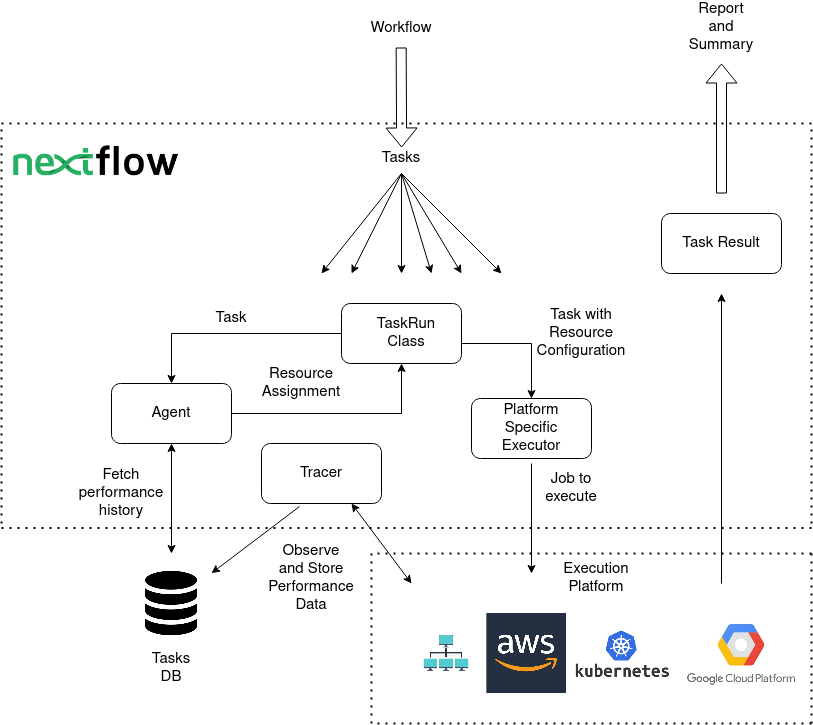
\includegraphics[width=0.8\textwidth]{fig/implementation_diagram.png}
        \caption{High Level Design: Integration of a Reinforcement-Learning Agent into Nextflow}
        \label{fig:implementation}
\end{figure}

Although the code for the reinforcement learning agents is logically a part of nextflow, when discussing the above design they will be referenced separately. The interaction between nextflow, the agents, and the external actors (the user, the database and the execution platform) is as follows. First, before a task is ready to be scheduled it is sent to a reinforcement-learning agent specific to that task, for the purposes of this thesis that was either a q-learning agent or a gradient bandit. Next, the task’s agent would then retrieve historical performance data and any other relevant data (i.e. what state the agent was last in) from the database. This database is external to nextflow and the creation and management of this database is not performed by nextflow or the agent which only use the database to save or read data beyond a workflow’s lifetime. Then, using the data, the agent selects a new resource allocation for the task and overwrites the task’s default configuration. After this, nextflow uses its custom executor for the given execution platform to prepare the task and pass it on to that platform. The task is then executed on the platform. It is important to note that the execution platform will also have its own system for managing, scheduling and executing jobs and processes. As the task is executed nextflow’s tracer module will gather performance data, i.e. peak CPU usage and peak RSS \footnote{https://www.nextflow.io/docs/}. Finally, once the task is finished all of this data is stored in the database for the agent to use the next time the task comes. It is important to note that there is one agent for each unique task. These agents are called whenever their task needs to be executed and they use the database to receive rewards for their previous actions.

Now that the structure of the agent’s environment has been explained and the relationship between collecting data and assigning a task resources is clear, it is time to delve into the specific approaches tried.

\section{Gradient Bandits}
\label{sec:gradient_bandits}

In the course of this thesis gradient bandits were used to allocate both CPUs and memory. The way they did this will be explained here.

\subsection{CPU Bandit}
\label{sub:cpu_bandit}

\subsubsection{Design}
\label{subsub:bandit1_design}

The CPU Bandit, as it was nicknamed, had a very simple set of actions to choose from which were based on the number of CPUs available to the system. The bandit then learned how many CPUs to allocate to its task. Its reward was a very straightforward function:

\begin{equation}
\label{bandit1_reward}
reward = -t\times(1+cpus - cpu\_usage/100)
\end{equation}


In this equation $cpu\_usage$ is a value in percent of the number of single core CPUs used by the task. If a task were assigned 4 CPUs and only effectively used two of them then $cpu\_usage$ would be $200$\%. $cpus$ is the number of CPUs assigned to the task and $t$ is how long the task took to run. Put in other words this equation punishes the agent with a negative reward equal to the amount of time it ran plus the unused CPU time (execution time multiplied by the number of unused CPUs). The idea is to provide an incentive for the agent to try to minimise the amount of time where any of the allocated CPU’s are not being used, and by punishing it with the amount of time that the task ran for, the agent is also encouraged to try to reduce the amount of time taken for the task to complete. This also means that, should a task have 100\% usage then its penalty is not 0 but is just the execution time. The reason for including time in the reward function is that if the agent has no concept of time it will always allocate the least amount of resources possible, since that is guaranteed to minimise the amount of resources wasted, and ultimately the tasks and their workflows would all be incredibly slow. 

\subsubsection{Picking the Right Step Size}
\label{subsub:const_stepsize}
The most pressing issue encountered with the CPU bandit approach was related to the step size. The initial step size $\alpha$ was $0.1$, which would be an appropriate step size for a bounded reward function with a mean reward that is around 10 or is known to have a standard deviation less than that (these values are based on the example given in \cite{sutton_barto} where they use a step size of 0.1 for a reward function with a statistical mean of 4). However the reward function used in \ref{bandit1_reward} has the bounds [ $-time \times (cpus+1)$ , $-time$ ] and as such is unbounded, since $time$ can be arbitrarily large and the standard deviation which was observed for the rewards was also too large. Therefore whenever tasks had a runtime $> 10$ seconds, $\alpha$ was too large. 

The danger in using a constant step size which is too large for the reward function is that when the bandit receives a reward which is considerably larger than the previous average the “step” taken in the direction of that action will also be too large and the bandits preferences will be updated such that the given action is always preferred and no other actions are tried any more. This causes the bandit to cease exploration too early. This effect was a common problem for tasks which took longer than 20 seconds to complete and was especially pronounced for tasks with runtimes of 100 seconds and more.  For these tasks the inherent volatility of the reward function relative to a step size of 0.1 meant that the bandits were converging very early and often had not explored the other actions at all. To provide a concrete example: if a bandit’s third allocation of CPUs received a reward of -150 and the first two allocations had had an average reward of -200, then for a step size of 0.1 the preference for the new allocation would increase by approximately $50\times0.1=5$. Now because of the exponential nature of the soft max distribution function used on the preferences, the probability of picking that action would increase by a large amount and then the bandit is in danger of converging to that allocation without any more exploration. This is best demonstrated graphically, as can be seen in figures \ref{fig:sub1} and \ref{fig:sub2}.

\begin{figure}[ht]
\centering
\begin{subfigure}{.5\textwidth}
  %\centering
  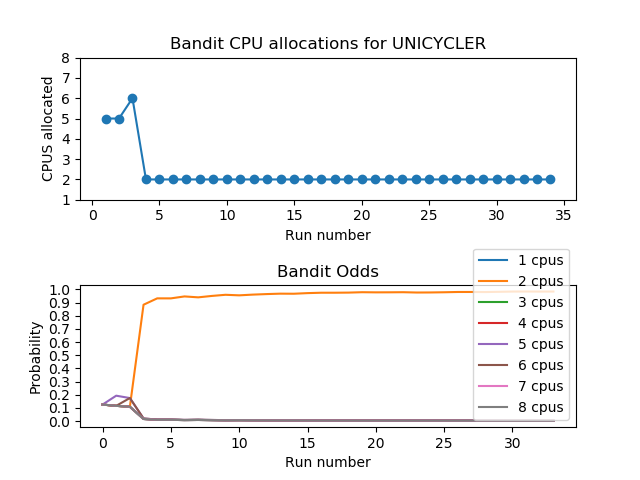
\includegraphics[width=\textwidth,height=\textwidth]{fig/old_UNICYCLER.png}
  \caption{Bandit 1}
  \label{fig:sub1}
\end{subfigure}%
\begin{subfigure}{.5\textwidth}
 % \centering
  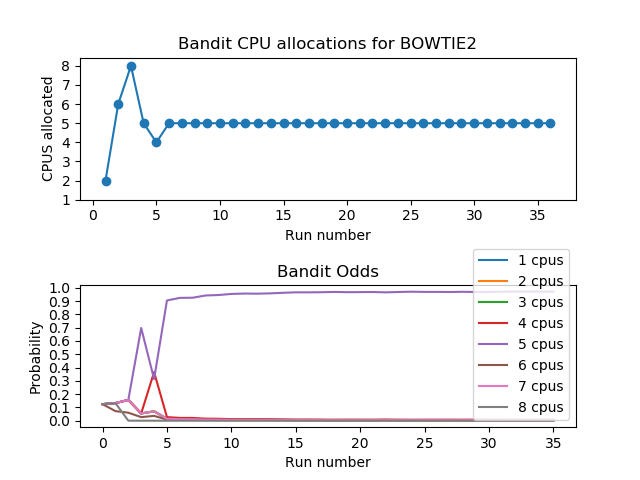
\includegraphics[width=\textwidth,height=\textwidth]{fig/old_BOWTIE2.png}
  \caption{Bandit 2}
  \label{fig:sub2}
\end{subfigure}
\caption{Example of Two Bandits Converging Too Fast}
%\label{fig:old_bandits}
\end{figure}

These figures show two gradient bandits which were exhibiting the behaviour described above. Each figure is made up of 2 graphs which display the action chosen by the bandit in the top graph and the probabilities for all of the actions in the bottom graph. As can be seen in the two examples, after receiving a relatively large reward, the agent’s probability of choosing a given action rises far too quickly and no other actions are attempted thereafter. This is occurring because the step taken by the bandit in the direction of a single action’s preference is too large and the resulting probability of choosing that action grows so much that no other actions are explored any more. 

The solution to this problem is to adjust the step size so that it is not a constant value but is instead a function which uses the average time that it usually takes the task to complete. This way tasks which have longer average runtimes are given smaller step sizes. The new value for $\alpha$ is thus $1/avg(time)$.

\begin{figure}[ht]
\centering
\begin{subfigure}{.5\textwidth}
  %\centering
  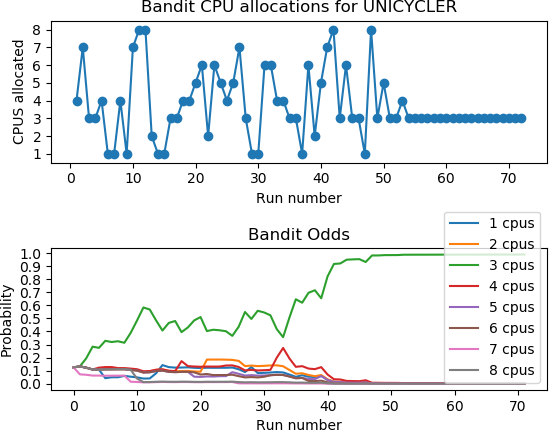
\includegraphics[width=\textwidth,height=\textwidth]{fig/UNICYCLER.png}
  \caption{Bandit 1}
  \label{fig:sub3}
\end{subfigure}%
\begin{subfigure}{.5\textwidth}
 % \centering
  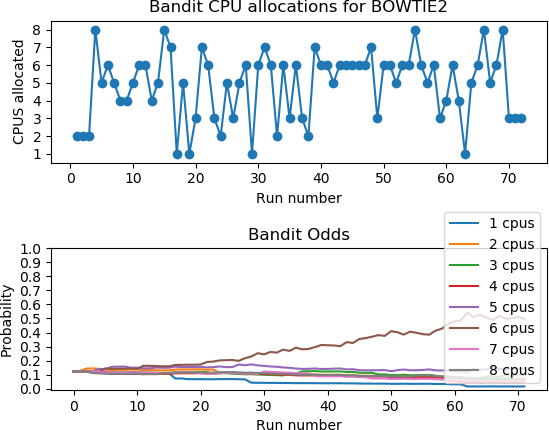
\includegraphics[width=\textwidth,height=\textwidth]{fig/BOWTIE2.png}
  \caption{Bandit 2}
  \label{fig:sub4}
\end{subfigure}
\caption{Bandits with a Step Size Based on Their Historical Average Execution Time}
\label{fig:fixed_bandits}
\end{figure}

The next two figures \ref{fig:sub3}, \ref{fig:sub4} show the same two tasks and their bandits but with the new step size. As can be seen the exploration phase is considerably longer and many different CPU allocations (actions) are tried before settling on one. Specifically in the case of the \textit{UNICYCLER} task’s bandit we can see that although allocating 3 CPUs seems to develop a strong preference early on (perhaps because it performed abnormally well once or perhaps because it genuinely is the best performing allocation) it does not become so preferred as to be dominant until much later and until that point the bandit continued to try other options.

It should be noted that these changes mean that for optimal performance of the bandits there should already be some historical data available about the task’s and their runtimes. It is not a necessity because over time the bandit can gather this data itself, but it is preferable.

\subsection{Memory Bandit}
\label{sub:mem_bandit}
The other gradient bandit approach used for assigning resources to tasks was called the memory bandit and its available actions were memory assignments. Beyond the obvious, the memory bandit was different from the CPU bandit in two respects. Firstly, the amount of memory available is several order of magnitudes larger than the amount of cpus. Thus, in order to limit the number of available actions to a manageable amount, the original amount of memory assigned to the task $m$ (in the default configuration) had to be split up into $n$ chunk,s each of size $c=m/n$. The bandit is then presented $a$ actions, each of which assigns $a\times c$ amounts of memory to the task. $a$ can be chosen as $1.5 \times n$ to give a good balance between considering allocations that are larger and smaller than the default configuration, however since it is known in advance that user estimates are usually quite poor one could also choose $a < n$ to encourage memory efficiency. In addition to this, by choosing larger or smaller $n$ values the size of the memory chunks can be adjusted. Secondly, and this is the biggest difference between the two bandits, a task which is assigned too little memory and overuses it will be killed. This means that there must be a special penalty for such cases.

The reward function used for the memory bandit, after assigning $memory$ bytes of memory is as follows:

\[ reward = 
\begin{cases}
   % \frac{x^2-x}{x},& \text{if } x\geq 1\\
    -2\times memory/c,& \text{if the task ran out of memory}\\
    -1 \times unused\_chunks              & \text{otherwise}
\end{cases}
\]

Where $unused\_chunks = (memory - peak\_rss) / c$ and $peak\_rss$ is the peak resident set size (RSS), in bytes, of the task during its execution.

An obvious alternative for this function is to simply use the memory usage: $reward = peak\_rss/mem$, and $\alpha = 0.01$ since the reward function’s range is [0,100]. However during testing this was found to be too small for tasks which have a low memory footprint. For example a task which uses 1\% of the assigned memory when assigned $n$ chunks, and thus receives a reward of 1\%, will only yield a maximum reward of $n$\% for the optimal allocation of just one memory chunk and for such small differences a gradient bandit will struggle to recognize the superior choice, even though it should be obvious. This is especially damaging to performance because these low usage tasks are precisely the ones where memory efficiency can be optimized the most and as such the reward function was changed to one which penalises the agent for the amount of unused memory. Of course to avoid the problem the CPU bandit had with its step size, the amount of unused memory in bytes could not be used and therefore the number of unused memory chunks was used instead. To return to the example of a task with 1\% usage that task’s rewards would now be $-n$ at worst and $-1$ at best, which makes it much easier for the bandit to determine good allocations. Finally in the case where a task has been killed the penalty is equal to double the number of memory chunks assigned because the agent must (at the very least) assign the same amount of memory again or must assign even more memory.

The actual implementation of the memory bandit is slightly adjusted so that whenever a task fails with one memory allocation and is retried with a new one, the new allocation must be greater than the previous one. If the bandit does pick a smaller allocation then it is ignored and the new allocation is either doubled or the default configuration for that task is used (if double the new allocation is also less than the failed allocation). This prevents the workflow from being broken off if a given task fails too many times due to repeated poor allocations.

Finally, to return to a discussion of step size similar to that in \ref{subsub:const_stepsize}, the memory bandit can be assigned a constant step size $\alpha = 1/n$. This is is because for $n$ memory chunks, the bandits reward function is bounded by [$-n$, 0]. 


\section{Q-learning Agent}
\label{sec:q_agent}

Similar to the approach with the gradient bandits, there was one q-learning agent per unique task. The q-learning agent’s state was always the current allocation of CPU and memory for the given task, and as its set of actions it could choose between incrementing or decrementing the amount of CPUs or memory, or it could do nothing. To limit the state space the maximum and minimum number of CPUs and memory as well as the amount by which they were incremented or decremented was based on the default allocation given to the task by the developers of the workflow (provided they did not exceed the resources of the execution platform). When the task was scheduled by the agent for the first time it would start in the default configuration’s state. Just like the memory bandit in section \ref{sub:mem_bandit} the possible memory states of the reinforcement learning agent are also chunks of memory. 

For the q-learning agent a different reward function was used than for the CPU bandit, primarily because it also had to incorporate memory but also as part of an attempt to experiment with different reward functions and approaches. 

\begin{equation}
\label{q_agent_1_reward}
r = -max(0.1,unused\_cpus) \times (t/avg\_t) \times (mem\times (1 - max(0.75,mem\_use)))
\end{equation}

Here the $mem$ variable refers to the memory allocated to the process and $mem\_use$ is the value of of the peak RSS of the task divided by the memory assigned to it. $avg\_t$ is a constant value which is determined at runtime based on the historical average execution time for the task. Lastly, $unused\_cpus = cpus - cpu\_usage/100$ where $cpus$ and $cpu\_usage$ are the same as in \ref{bandit1_reward}. 

Since division by the task’s average time is incorporated into the reward function it did not need to be incorporated into the step size as with the gradient bandit (see \ref{subsub:const_stepsize}) and the issues associated with that were avoided. This function is effectively a product of the number of unused CPUs, the slow-down factor and the amount of unused memory. However there are some slight modifications. The $max$ function is used to set an artificial floor for the penalty incurred by the unused CPUs and unused memory. Tasks which use more than 90\% of the available CPUs are given the same reward as tasks which use exactly 90\% in an attempt to prevent the agent from deciding to assign each task 1 CPU in order to minimise the number of unused CPUs. Additionally the floor for unused memory is capped at 25\% in a similar manner. This is done to discourage the agent from allocating too little memory because tasks which use too much memory will of course be killed and have to start over, which can have a detrimental effect on performance. This reward function is of course negated in order to turn it into a penalty function so that the agent will seek to minimise its penalty by minimising the number of unused CPUs, the slowdown and the amount of unused memory.

The q-learning agent also has 3 other parameters- the step size $\alpha$, epsilon $\epsilon$ and the discount $\gamma$. Step size was set to 0.1 and the discount was 1.0. Epsilon is adjusted over time- at first it is 0.5, to encourage exploration, then after 50 runs it is decreased to 0.25 and after 100 runs it is 0.1 to discourage exploration but leave room for the bandit to still occasionally try other actions and visit different states.

\subsubsection{Exploring the State-Action Space}
\label{subsub:states}

It should be noted here that unlike the gradient bandits from before, which had to decide from $c$ or $n$ number of actions for the CPU and memory bandits respectively, the q-learning agent must learn the value function for $(c-2)*((m-2)*a + 2*(a-1)) + 2*((m-2)*(a-1) + 2*(a-2))$ state-action combinations. Here $c$ is the number of possible CPU states, $m$ is the number of possible memory states and $a=5$ is the number of possible actions. Now since the q-learning algorithm from \ref{alg:q-learning} needs to try each action in every state combination at least once, and explores with probability $\epsilon$ then for arbitrary examples of $c=4$ and $m=3$ it will take, at the very least, 46 different runs just to have tried every action in every state once. This shows how much more complex the q-learning approach is than the gradient bandit approaches. Ultimately however the theoretical benefit posed by q-learning is that when the agent learns, for example, not to increment the amount of CPUs when in state $s$ (where $s$ is also the number of CPUs currently allocated), the agent is thus also learning to avoid all states/allocations $\{s_c \in S$ $|$ $s_c > s\}$ which allocate more CPUs than $s$. While this seems trivial, the gradient bandit is unable to see such connections and cannot tell that a task which has low CPU usage for $s$ CPUs can be expected to have even lower usage for $s_c > s$ CPUs. 



%!TEX root = ../thesis.tex

\cleardoublepage
\chapter{Evaluation}
\label{cha:evaluation}

This chapter reviews how the approach from the previous chapter was tested, and discusses the observed results. This chapter will explain the setup of the testbed, as well as the motivation behind the types of tests which were performed. Finally a discussion of the results and their origins will take place.


\section{Approach to Evaluating Performance}

In order to evaluate the success of the proposed approach a multipath scenario with four links will be emulated and investigated. Each test will consist of two WAN connectors, and the four emulated links going between them. The characteristics of the links will be changed during the tests, each time with respect to different properties: latency, packet loss, and jitter. The evaluations will be performed on a testbed consisted of four seperate host servers. Two of these servers will act as the originating and terminating WAN Connectors. One server will generate and measure traffic, in between the two WAn Connectors, a server will act as the link emulator. This architecture is shown in figure \ref{fig:testbed}

\begin{figure}[h]
    \centering
        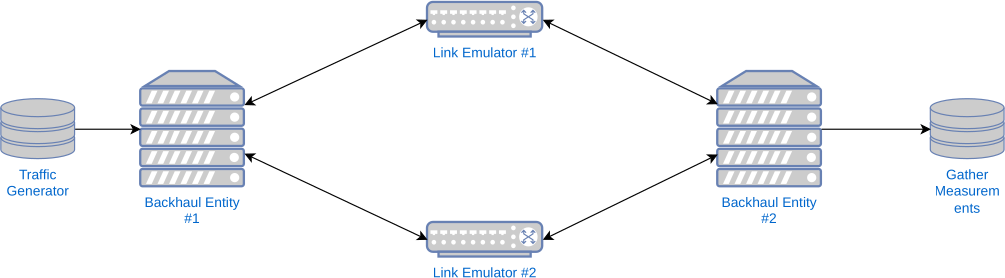
\includegraphics[width=0.66\textwidth]{fig/testbed.png}
        \caption{Testbed Setup}
        \label{fig:testbed}
\end{figure}

In figure \ref{fig:testbed}, the links between the servers are 10 GB ethernet cables. The hosts are connected as is shown. In the "traffic generator and measurer" two linux namespaces are used to separate the traffic generation and the measurement. The packets generated in one namespace are routed via the ethernet connection to the next host (the terminating or "edge" WAN Connector), because of the linux namespace they are not aware that their destination is technically the same host. The packets are then are backhauled by the WAN Connector over the emulated links in the next host, and via the terminating WAN Connector, back to the original host, but now in the "measurer" namespace.

The link emulation is done using the tc subsystem. First a root Heirarchical Token Bucket qdisc is established on the "downlink" and "uplink" interfaces (the ethernet cables between the WAN Connectors). In this case, the link emulation is performed before the outoing packet is queued on the ethernet cable, so that is also where the qdisc is placed. Secondly, the qdisc is given children classes, one class per link. This allows one to establish bandwidth caps for each emulated interface. Within these HTB classes the root qdisc is a netem qdisc. These allow the installation of link characteristics such as latency, packet loss, and jitter.

%In all of these scenarios the same traffic flows will be replayed. This traffic will contain different types of flows, with different QoS requirements. Before a new flow is started, the flow's requirements are sent to the WAN connector and it is either accepted or rejected. During the traffic replay, the delay, jitter, and reliability will be measured.

%All of these tests can be performed on the same testbed which will be set up as is shown in Figure \ref{fig:testbed}. The testbed architecture features a traffic generator, two WAN connectors, with a link emulator between them, and a measurement module to analyze performance. In practice the traffic generator and the test bench will be co-located on the same machine. The link emulator, and the WAN connectors are separate hosts, all interconnected over ethernet. The link emulation is done using the linux kernel's traffic control subsytem (TC). TC offers a network emulator (netem) queuing discipline (qdisc), which is able to emulate various link characteristics including delay, jitter, packet loss and packet re-ordering. Furthermore by combining the netem qdisc with a rate limiter, such as the Heirarchical Token Bucket (HTB) qdisc, a link can have its bandwidth limited. This allows one to emulate links with different latency, reliability and jitter, and with different maximum bandwidths.

In order to make the emulation more realistic, the netem qdiscs will periodically be adjusted, this allows one to degrade or improve links over time, for example by increasing the latency or packet loss in frequent intervals, up to a large value. It also more closely mimics the real-life behavior of WAN connections, which do experience changes in their characteristics over time.

For the purposes of evaluating the WAN connector, three series of experiments will be performed to isolate and investigate it's link switching capabilities. First, purely latency based link selection will be investigated- a flow will be defined with specific latency requirements and then the emulated links will have their latency repeatedly changed. The same will be done once with packet loss and with jitter. In each of these scenarios the other two parameters will be held constant, so that the WAN Connector can be judged based on its ability to meet one of the latency, jitter, or packet loss requirements, without the other two requirements interfering. In order to simulate realistic scenarios these experiments will also be repeated once with background traffic which aims to saturate the link's capabilities.

The data for the emulation used in all of these scenarios was obtained using the Satellite Constellation Network Emulator (SCNE) \footnote{https://connectivity.esa.int/projects/scne} from the European Space Agency. The default scenario is 24 hours long and consists of 288 satellites, 10 gateways (GW), and 50 user terminals (UT). The reason this data is used is because LEO satellite links are expected to be the most common type of backhaul link for geographically distributed 5G Campus Network deployments. Furthermore, since LEO satellite connections are exceptionally more volatile than "regular" links \cite{deutschmann2022broadband} \cite{ma2023network}. By choosing to emulate more volatile links in the testbed, the WAN Connector experiences a more difficult test, and one can be assured that the real life performance in "normal" scenarios, is highly unlikely to be worse.

Since the WAN Connector is defined to work on at most four outgoing links, each investigated scenario will feature four links. These links will all be based on data from the SCNE emulation.

\subsection{Accuracy of the Emulation}

To make sure that the testbed emulation also matches the values from the SCNE, a brief comparison was done, where the testbed's latencies were compared with those recorded in the SCNE. 

Figure \ref{fig:sim_vs_em} shows the comparison between the data observed in the testbed, and the SCNE. The testbed data in the graphic is measured by the packet flows running over the individual links. The emulation data comes from the values recorded during withh the SCNE. Since the testbed data is collected at a rate of 100 packets per second, but runs at 10 times the speed of the SCNE emulation, there are 10 times as many data points. This explains why the testbed data appears blurrier.

\begin{figure}
  \centering
  \begin{tabular}{@{}c@{}}
    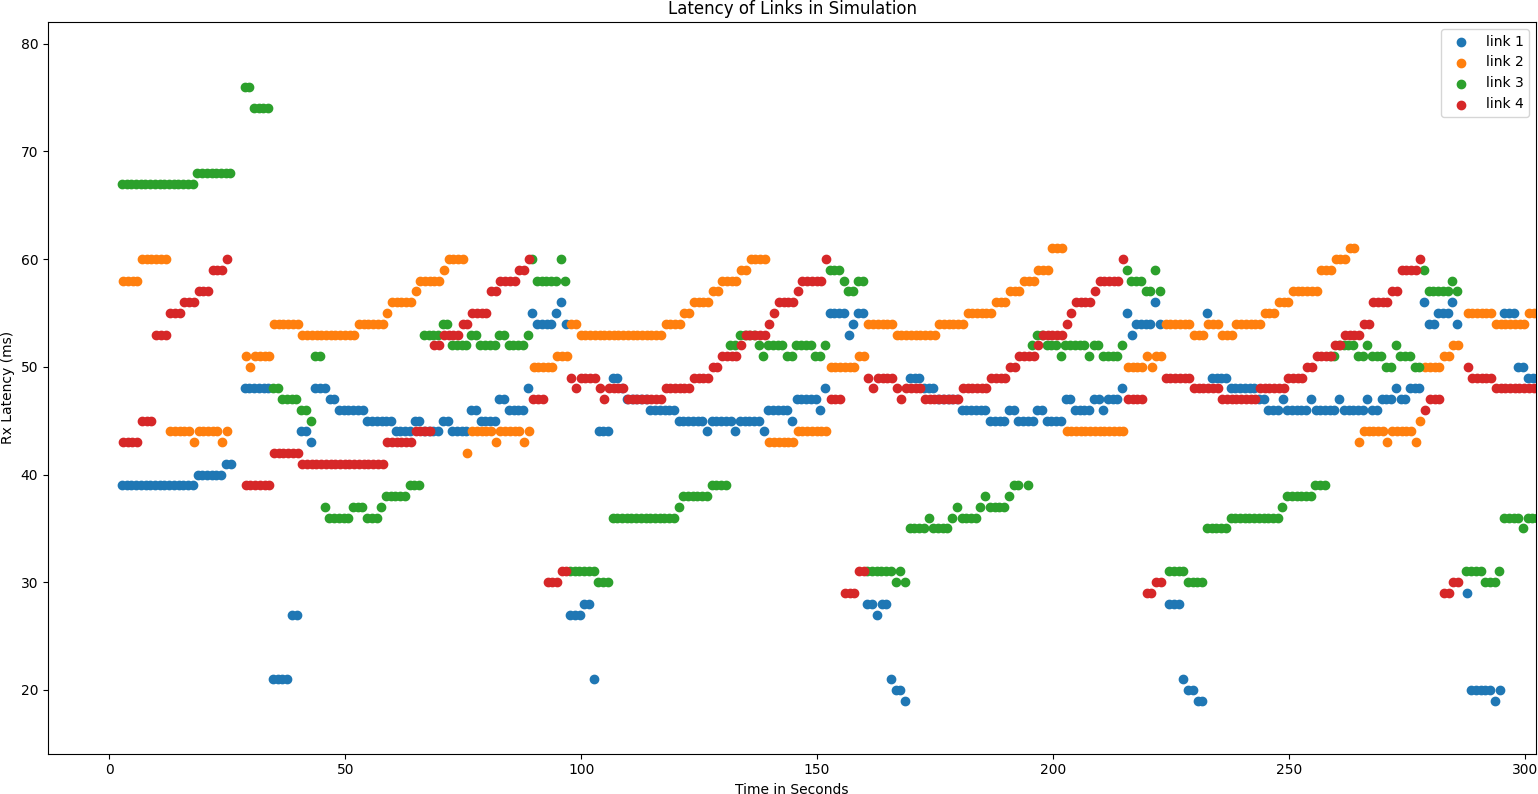
\includegraphics[width=\linewidth]{fig/simulated_latencies.png} \\[\abovecaptionskip]
    \small (a) Latencies Recorded in SCNE
  \end{tabular}

  \vspace{\floatsep}

  \begin{tabular}{@{}c@{}}
    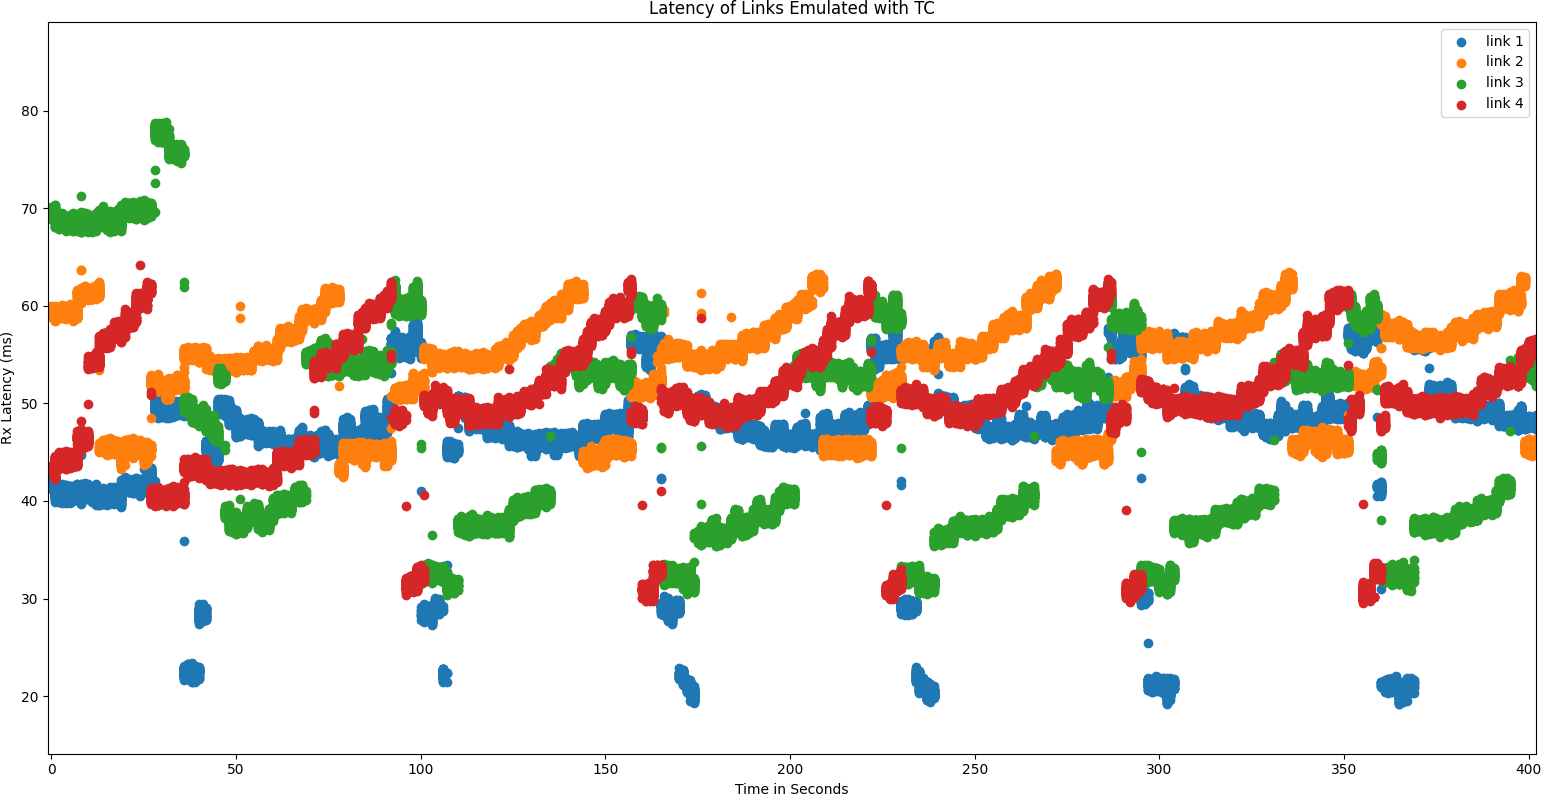
\includegraphics[width=\linewidth]{fig/emulated_latencies.png} \\[\abovecaptionskip]
    \small (b) Emulated Latencies Measured in the Testbed
  \end{tabular}

  \caption{Comparison of the Emulators Latencies and the Testbed}\label{fig:sim_vs_em}
\end{figure}

As can be seen in the figure \ref{fis:sim_vs_em}, the latencies recorded on the testbed closely match those from the SCNE, which it was seeking to replicate.

\section{Latency Based Path Switching}

First is the scenario investigating latency. During the emulation, the simulation data is used to adjust the tc netem qdisc on the "link emulator" machine periodically. Because the SCNE simulator provides latency data over a 24 hour period, in 10 second intervals, the simulation data is "sped up". That is the emulation is changed each second, based on the next datapoint from the simulation. This means the 24 hour window can be run over a 2 hours test. Since real links are usually steadier and less volatile than the sped up emulation one can expect results in a real situation to be better.

In the experiment 100 packets are sent per second across each link, as well as 100 packets per second from the traffic generator, through the WAN Connector. This is done to have a comparison between the performance of the WAN Connector and the baseline performance level, which would be the best performing link. In any scenario the minimum acceptable performance of a path switching application would be to provide a better performance than the best single link. Otherwise it would be better to just select the best link, and not use the application at all.


\subsection{Performance Compared to Single Links}

For the experiment a flow is defined in the WAN Connector with a minimum round trip time (RTT) of 56 milliseconds. This value is chosen because it is the mean of the mean values of the latencies of the four links from the emulation. For the evaluation of the latency based path switching a single flow matching the definition stored in the WAN Connector is backhauled through the WAN Connector at a rate of 100 packets per second. In order to serve as a comparison, identical 100 packet per second flows are sent across the four other links. Finally their latencies are compared, and the latencies measured by the four links are used to calculate the Oracle approach.

The graphics \ref{fig:latency_cdf1} and \ref{fig:latency_cdf1_super_zoomed_in} show a cumulative distribution of the different latencies experienced by the packet flows running over the individual links and the WAN Connector, as well as the performance of the Oracle approach. The Oracle results are purely theoretical. For each packet, it is able to select the best link to forward on, based on that links future characteristics. This approach is calculated by comparing each packet sent by the WAN Connector with the latency that packet \textit{would} experience on any of the other links, and if the latency of the WAN Connector's link would be greater than the minimum value (56 ms), selecting a different link (if one exits) with a lower latency. Since it always picks an optimal path, the Oracle approach provides an upper bound on the best possible performance. In practice it is not possible because it has knowledge of the future, but nonetheless it acts as a very valuable comparison.

\begin{figure}[h]
    \centering
        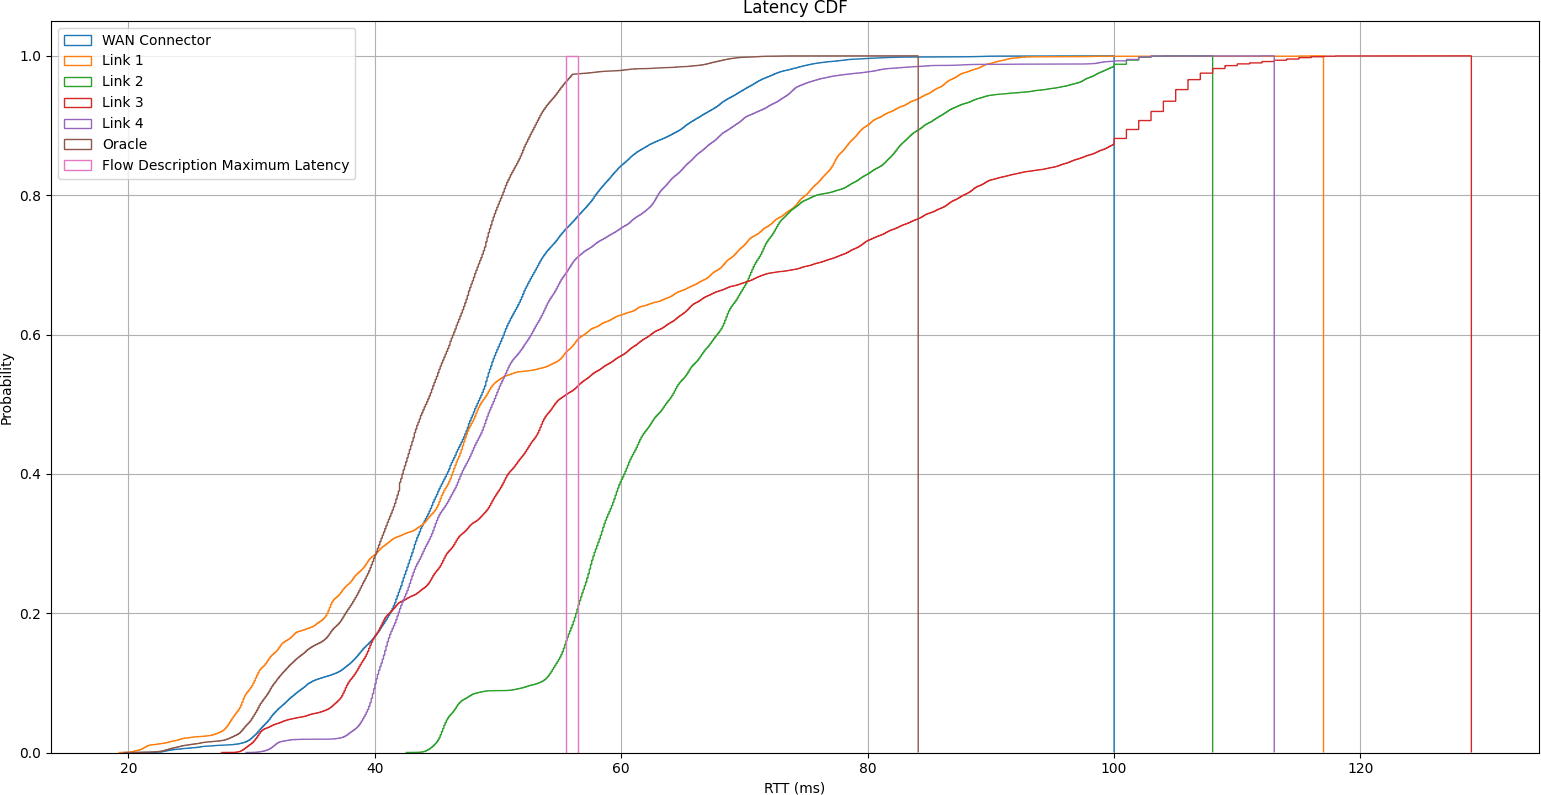
\includegraphics[height=0.8\textwidth,width=\textwidth]{fig/latency_cdf1.png}
        \caption{Cumulative Distribution of the Latencies}
        \label{fig:latency_cdf1}
\end{figure}

\begin{figure}[h]
    \centering
        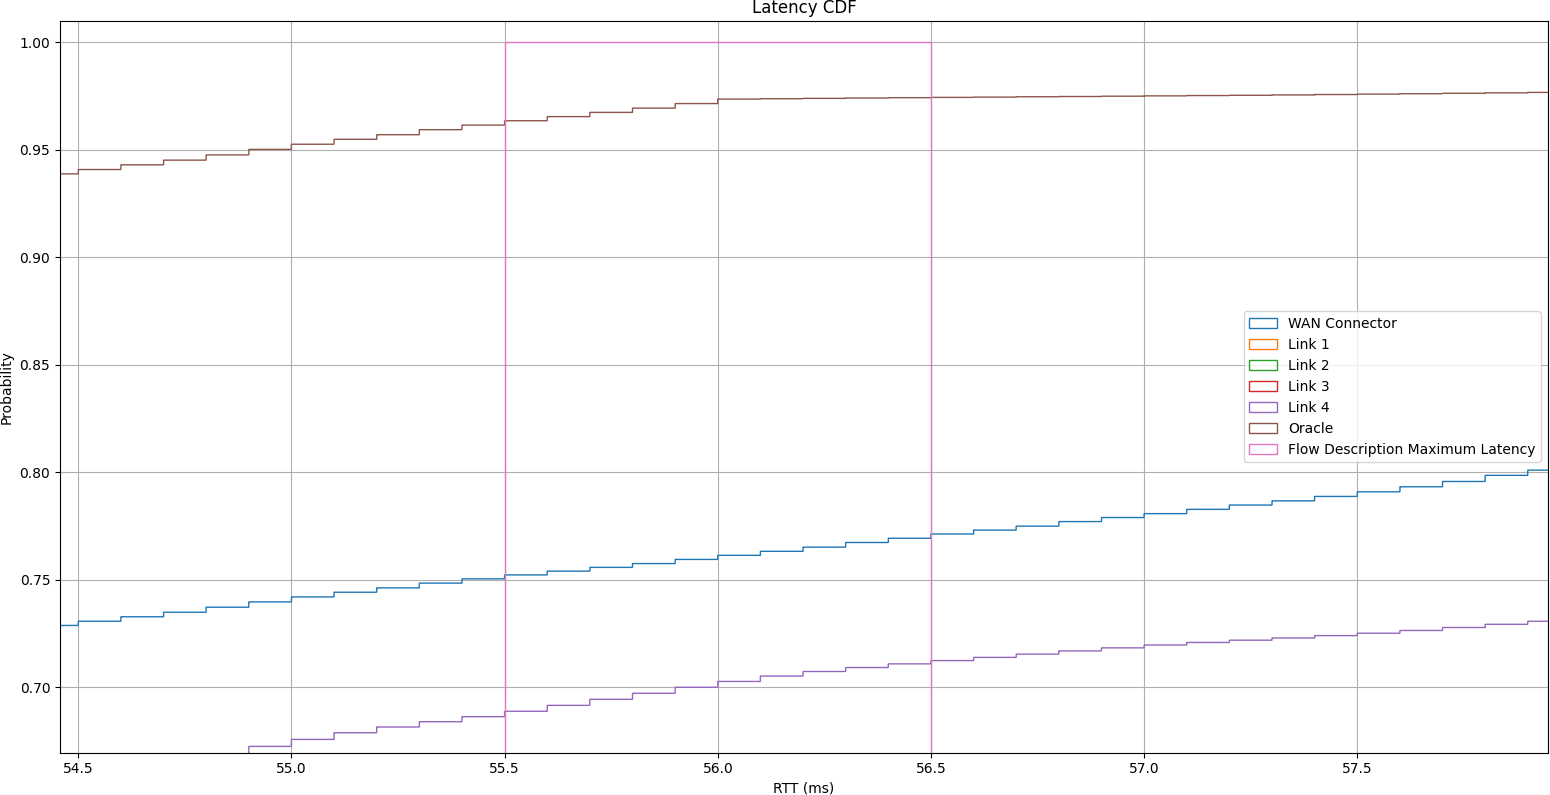
\includegraphics[height=0.66\textwidth,width=\textwidth]{fig/latency_cdf1_super_zoomed_in.png}
        \caption{Closeup of the Latency CDF}
        \label{fig:latency_cdf1_super_zoomed_in}
\end{figure}

The CDF shown in figure \ref{fig:latency_cdf1} and zoomed in on in figure \ref{fig:latency_cdf1_super_zoomed_in} tracks the probability that the flow experiences a latency less than or equal to the latency value on the y axis. The pink bar labelled "Flow Description Maximum Latency" is set at 56 milliseconds and represents latency bound for the flow being measured, which was communicated to the WAN Connector.


The results in the figures show that the WAN Connector is able to achieve a superior performance to any of the individual links on their own. This was the baseline requirement and it is important that it is able to achieve this. However the performance does not significantly improve on the next best link, which is is able to achieve the maximum allowed latency 72\% of the time, while the WAN Connector does so 77.5\% of the time. The Oracle approach shows that in theory one could, at best, have maintained the minimum latency required by the flow in 95\% of the cases. This means the WAN Connector's performance is only 80\% optimal.


\subsection{Latency Performance Under Load and the Importance of Traffic Shaping}

During this experiment, the same 100 packet per second flow from before is repeated, but background traffic is added. An iperf3 test is run across the WAN Connector at the same time as the latency critical flow, and the background traffic is given the same latency requirements, so that the WAN Connector always schedules both flows to the same link. This ensures that whatever link is being used will be saturated. Latency performance during congestion and close to congested scenarios is a crucial element of a deterministic backhaul solution. The WAN Connector's control plane only makes decision about which link to forward on- it does not perform load balancing or prioritization. The data plane does not do this either, it implements a purely First In First Out (FIFO) approach to packet queuing. This is done because the burden of implementing an appropriate packet shaper, in addition to the other multipath calculations, is too significant for the purposes of this thesis, and because very powerful traffic shaping implementations, which are easy to integrate into this solution, already exist.

\begin{figure}[h]
    \centering
        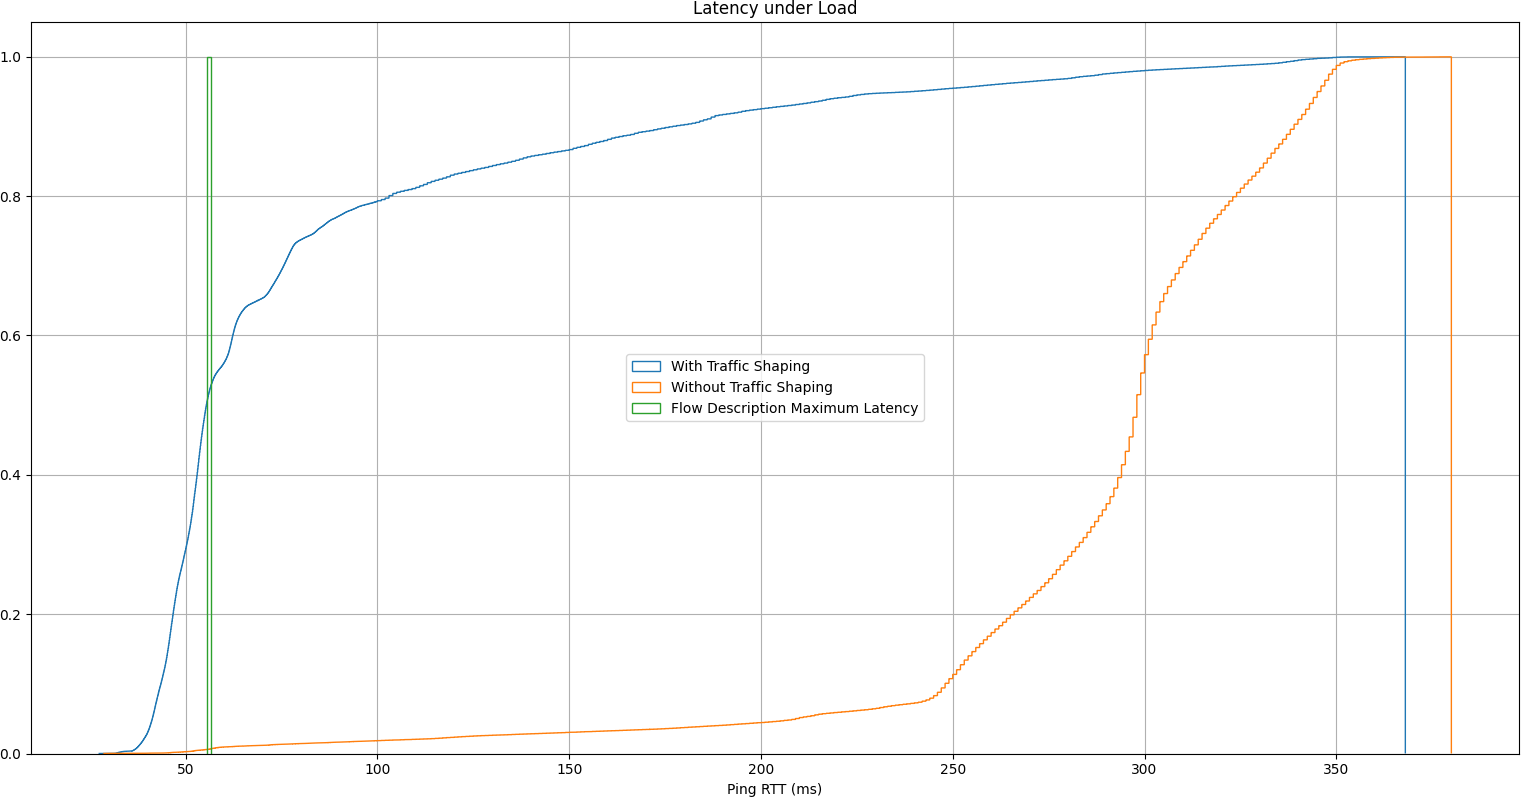
\includegraphics[height=0.66\textwidth,width=\textwidth]{fig/rrul_cdf.png}
        \caption{Latency with Background Traffic}
        \label{fig:rrul_cdf}
\end{figure}

The figure \ref{fig:rrul_cdf} neatly demonstrates why traffic shaping is an essential element of any deterministic network. In the case in which there is no traffic shaper the latency critical flow experiences significant additional latency due to the network being overloaded. The TCP algorithm fills the link's capacity, and the latency critical packets spend too much time buffering and arrive late. It should be noted that the WAN Connector's performance with the traffic shaper is worse than in the previous scenario, where there was no background traffic, and only 50\% of the packets are under the required latency of the critical flow. However the approach without the traffic shaping is at just 1\%.

\section{Reliability Based Path Switching}

In the next scenario, to analyze the ability of the WAN Connector to achieve the required reliability of a given flow, the same test flows from before are run over the WAN Connector and the four outgoing links. However this time instead of varying the latency, the packet loss ratio of the link is changed. The SCNE emulation's data is used for the testbed once again. However since the emulation does not provide packet loss on a per second basis, the latencies of all the different links in the simulation are used. For the emulation, these 51 values are looped over in 10 second increments. Each link is given a shuffled set of these 51 values. This means that the cumulative value of the packet loss experienced by all of the links is the same (2\%), but the instantaneous values will differ. To appropriately analyze this scenario the flow being backhauled over the WAN Connector is given a reliability threshold of 0.1\% this is because in this scenario, where the existing links all provide an average of 2\% reliability, it becomes necessary to duplicate at some points, in order to achieve the required reliability. Afterward, the experiment is repeated under load, like in the latency scenario, where the test flows across the links themselves are not run, and a second iperf3 flow is run across the WAN Connector in order to saturate the link. Like before, this second flow is given the exact same requirements as the test flow, in order to ensure that they are always running across the same link.

 The results of this experiment are shown in figure \ref{fig:loss_bars1}. The packet loss recorded by each of the flows over the period of the experiment is plotted in a bar graph, as well as the theoretical packet loss which would have been experienced by the Oracle approach.

\begin{figure}[h]
    \centering
        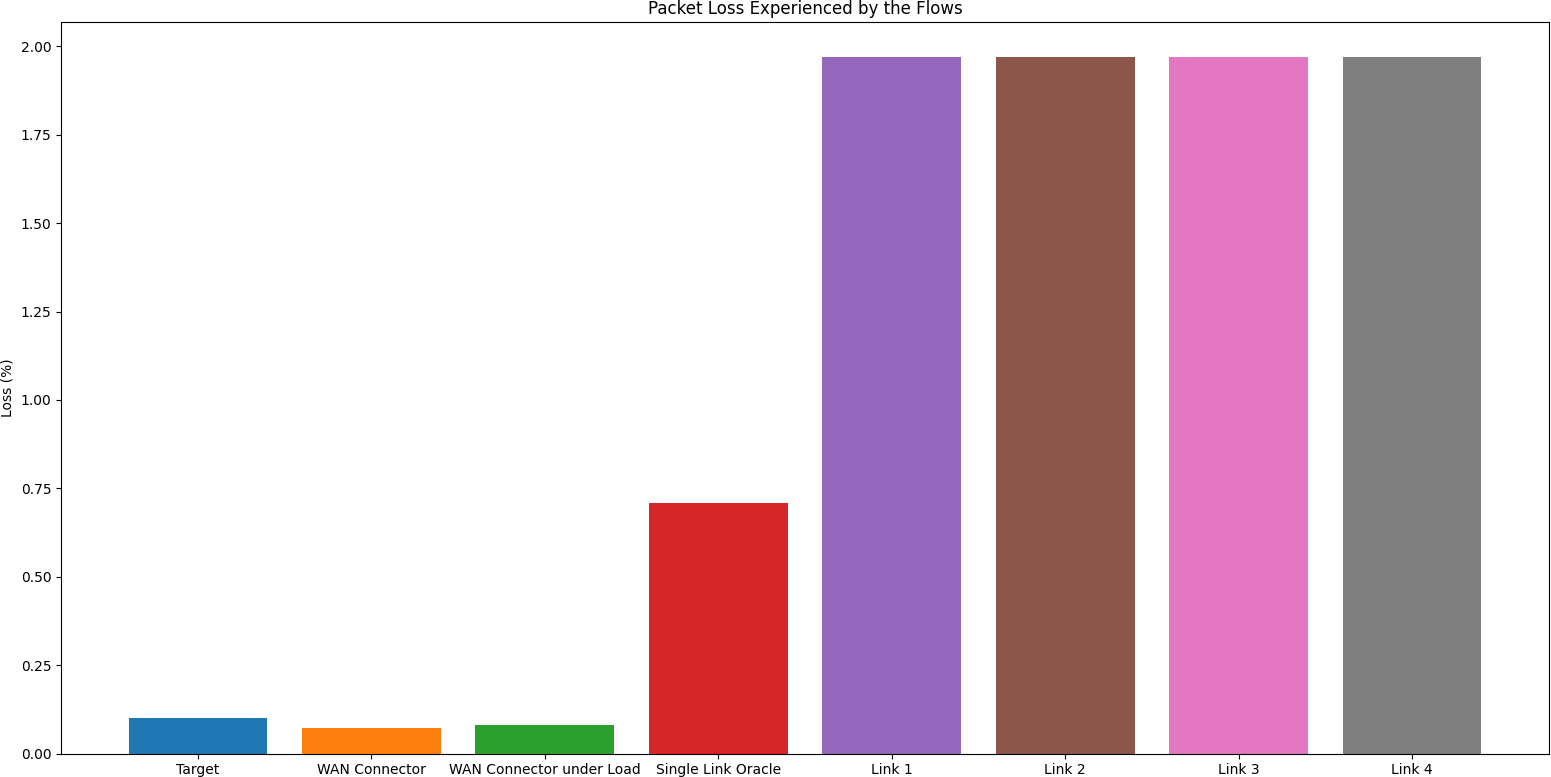
\includegraphics[height=0.66\textwidth,width=\textwidth]{fig/loss_bars1.png}
        \caption{Reliability}
        \label{fig:loss_bars1}
\end{figure}

For the analysis of the performance this time the Oracle approach is defined as choosing, before forwarding any packet, the link with the lowest packet loss ratio. But, crucially, the Oracle is not allowed to duplicate flows across different links. This explains why in figure \ref{fig:loss_bars1} the Oracle is outperformed by the WAN Connector. Indeed, as the graphic shows, it is not possible to achieve the critical flow's required reliability with any of the available links, nor with the Oracle approach. But the WAN Connector is able to achieve it. This speaks to the potency of the flow duplication approach, which is made possible in the optimization equation used to decided on which flows to forward.

\subsection{Impact on Throughput}


\begin{figure}[h]
    \centering
        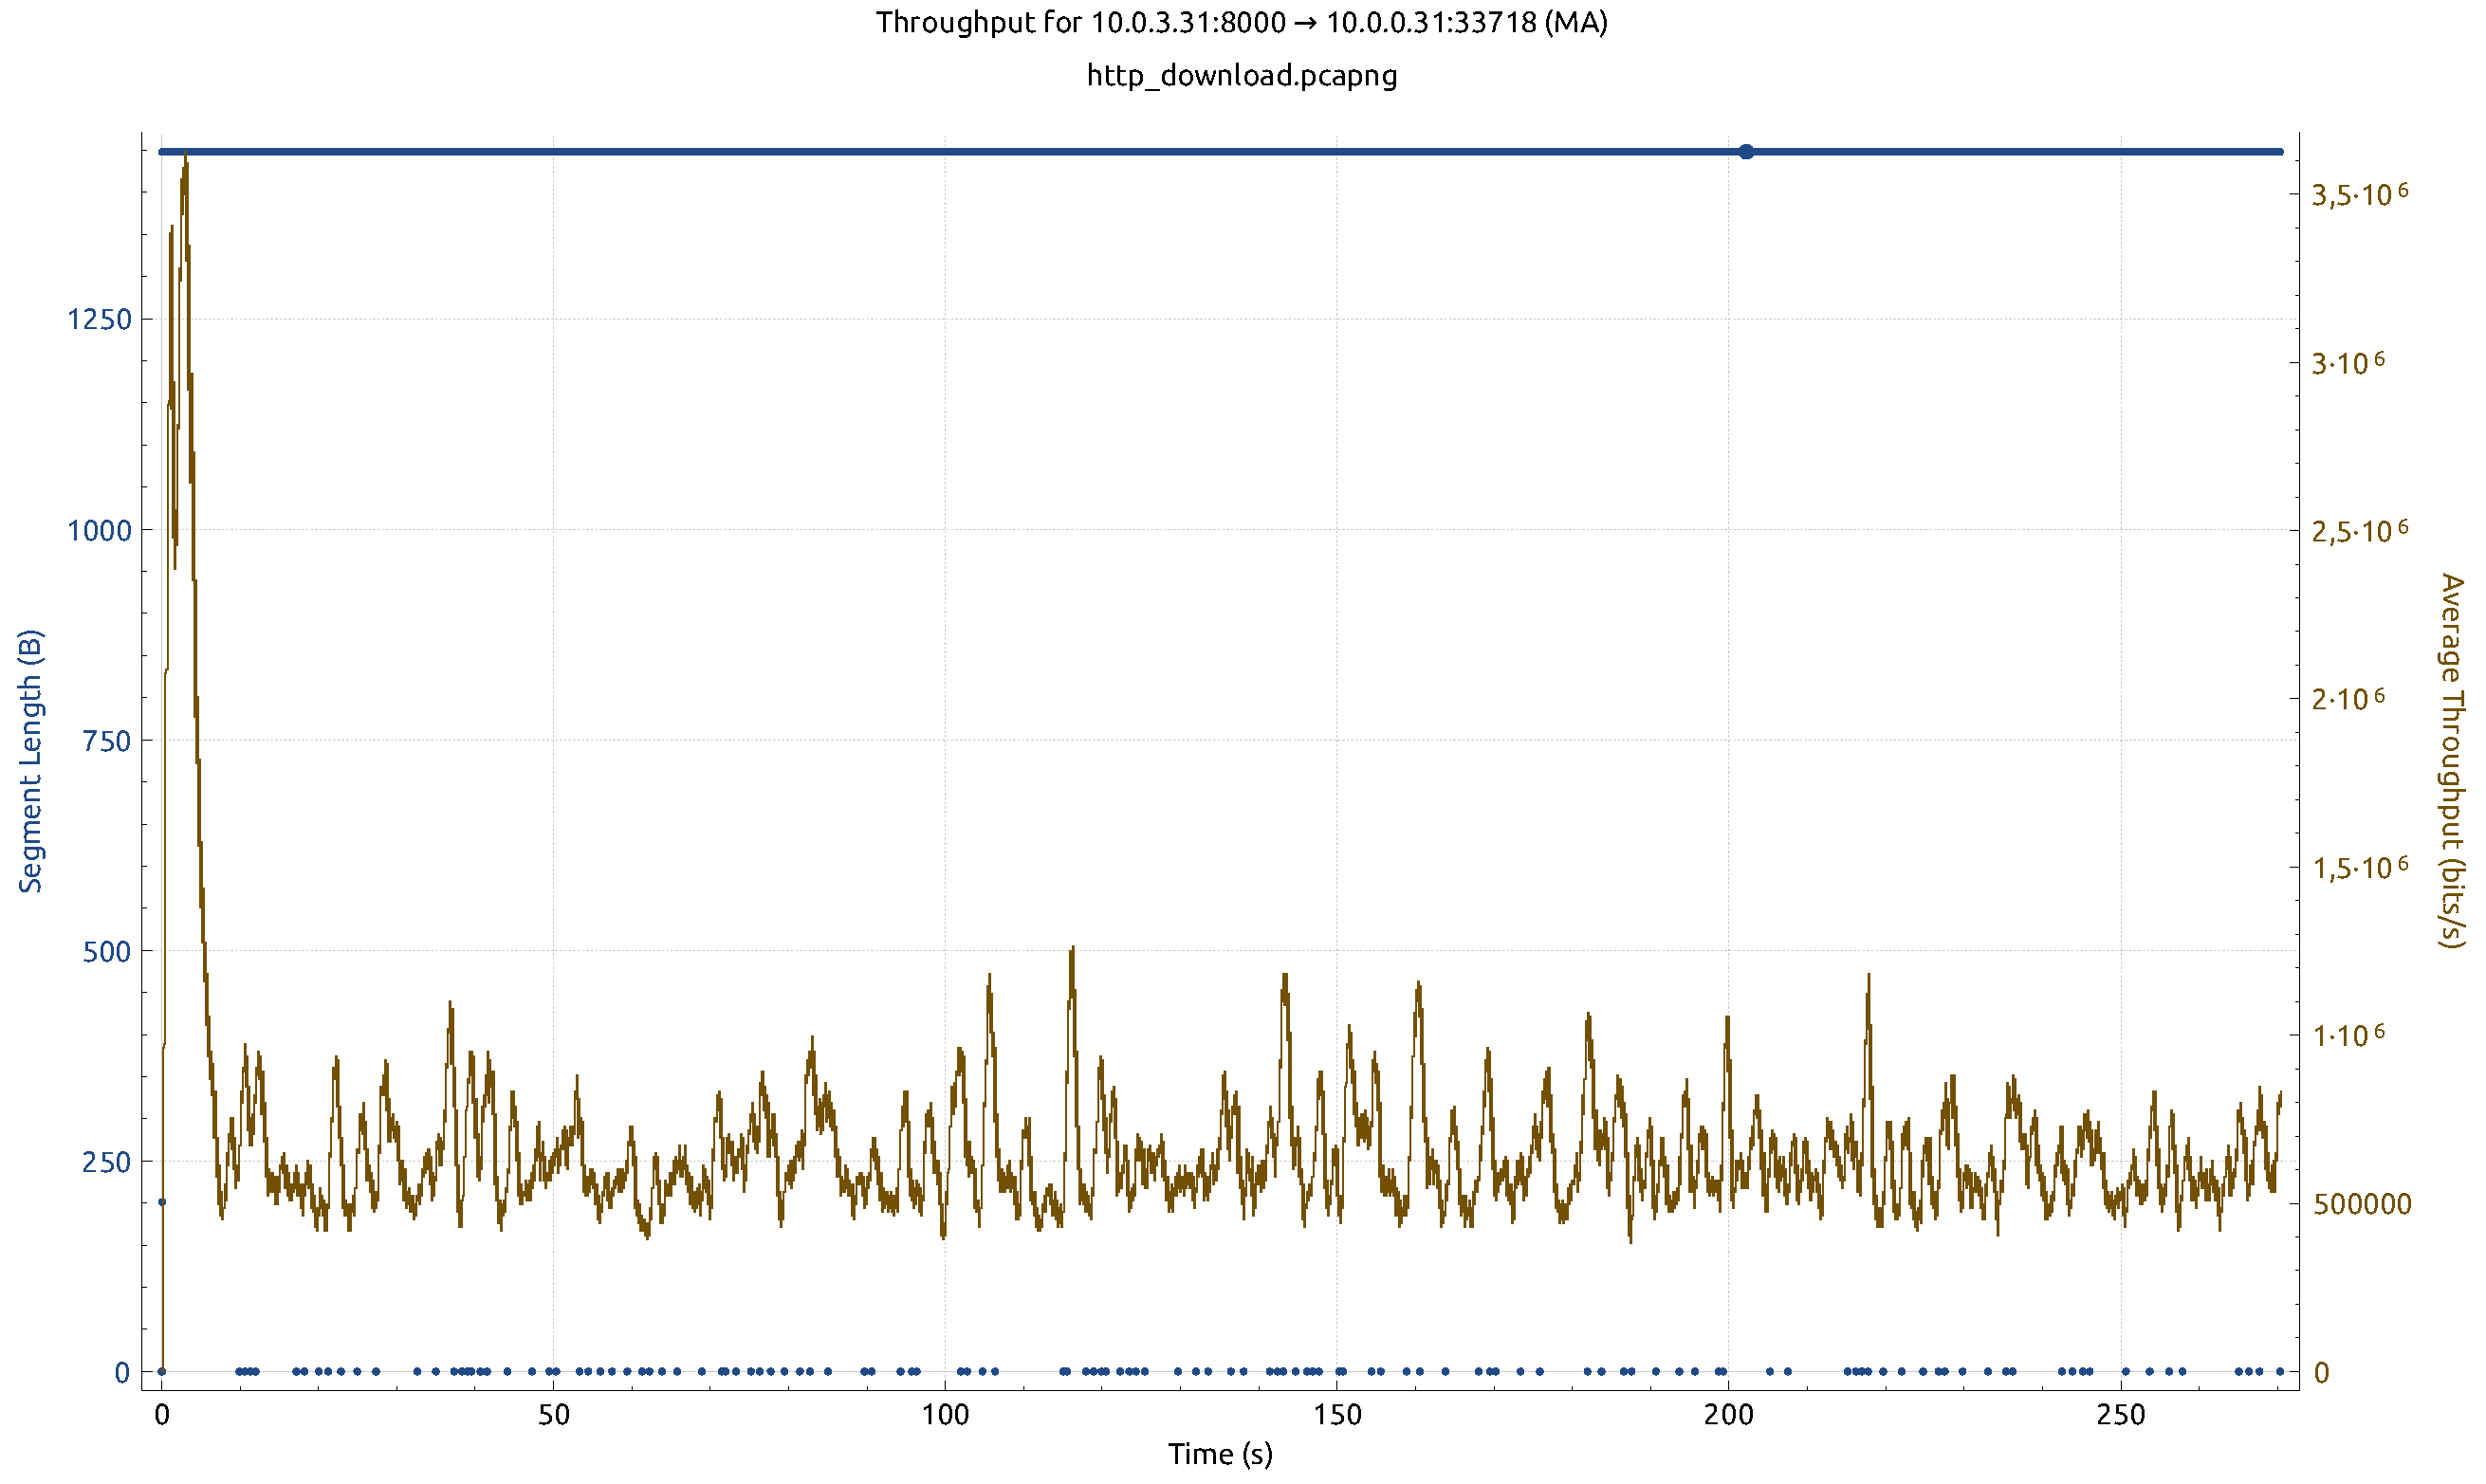
\includegraphics[height=0.66\textwidth,width=\textwidth]{fig/tcp_throughput.pdf}
        \caption{Throughput of a Duplicated Flow}
        \label{fig:dup_tcp}
\end{figure}

One of the unfortunate impacts of packet duplication is that it reduces the available bandwidth. It represents a waste of up to 50\% of the available resources, in the worst case, where every flow must be duplicated. Additionally, since flows which are being duplicated need to be re-ordered, this means that the FIFO approach for packets cannot be used and instead the packets must pass through a Packet Ordering and Elimination Function (POEF). When a packet arrives out of order the POEF starts to incur significant additional overhead because it must store all packets until the missing packet arrives, or a point is reached at which the stored packets must be dequeued. This point is either the point at which the packets expire, or the queue of out of order packets becomes full. Beyond this, the storing and eventual mass de-queuing of out of order packets can also interfere with the TCP algorithm- thus leading to reduced throughput.

These two effects - the POEF overhead and it's effects on TCP- lead to a very heavily reduced throughput, as can be seen in figure \ref{fig:dup:tcp}. The graph in the figure shows the throughput experienced by a routine TCP download, running over the WAN Connector, and experiencing replication, as well as the segment length of the TCP stream. As can be seen in the graph, the throughput is very low, and is not able to saturate the link's bandwidth despite being the only flow running at the time.

\section{Jitter Based Path Switching}

\begin{figure}[h]
    \centering
        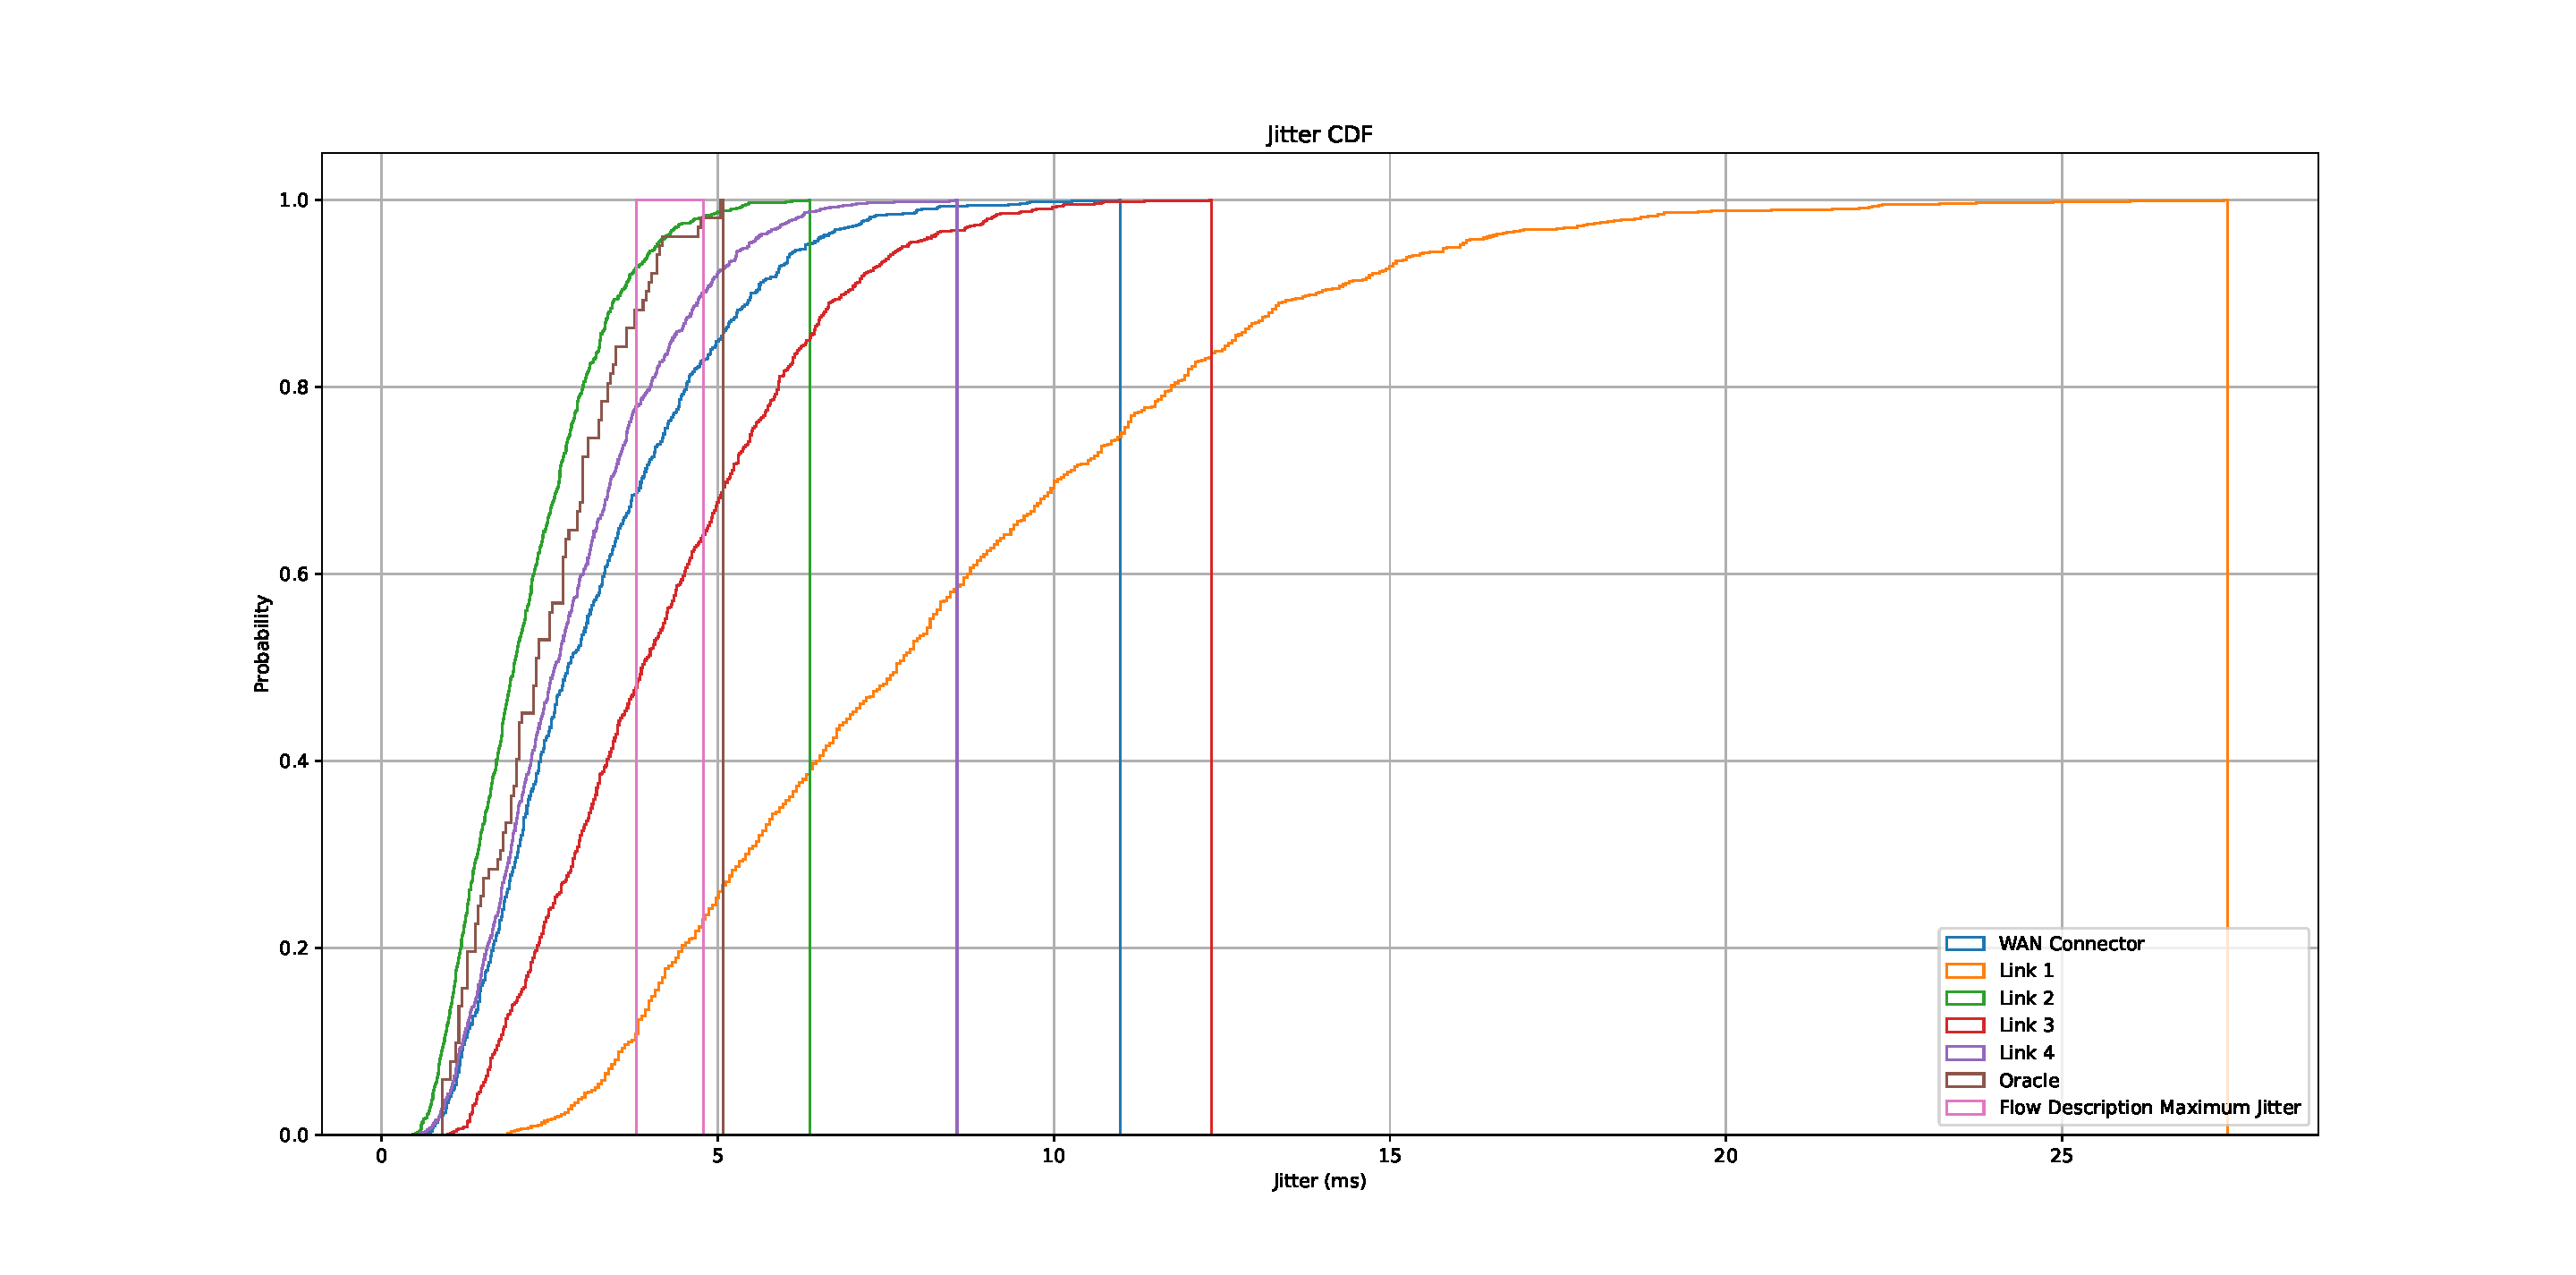
\includegraphics[height=0.66\textwidth,width=\textwidth]{fig/jitter_cdf.pdf}
        \caption{Performance of Jitter Based Path Switching}
        \label{fig:jitter_cdf}
\end{figure}

For the final analysis, the jitter must be investigated. For this purpose the simulation data was once again adapted. This time the standard deviation of the latency experienced was calculated for each of the 102 connections in the simulation. Then these standard deviations were scaled down by diving them by one, two, three, and four, respectively, in order to acquire four different set of jitter characteristics. Finally the scaled values were shuffled. This resulted in 4 links with varying jitter characteristics, which suffices for the emulation. Each different jitter value is emulated for 10 seconds on the respective link. During the emulation scenario a UDP iperf3 stream is ran at a rate of 3/4ths of the link's capability for 1000 seconds. iperf3 records jitter each second, and this data is used to then analyse the performance. Since more than half of the link capacity is being used by the flows being sent on the links (and not through the WAN Connector), the WAN Connector cannot be tested at the same time. Thus, to test the WAN Connector the emulation is repeated but with the flow only being sent over the WAN Connector. Lastly, the Oracle approach is calculated based on the simulation data. The Oracle approach, like before, displays the theoretical optimal performance. It chooses, at each point in time, the link with the lowest jitter. The cumulative distribution of the jitter experienced by the flows is plotted in figure \ref{fig:jitter_cdf}. 

As can be seen from the figure, the WAN Connector gave a very disappointing performance. It displays an inferior performance to two of the links. This means the path switching is actually causing a worse performance. This is most likely down to insufficient statistics causing poor path selection, because jitter statistics can't be gathered about other paths in this single flow scenario. The probe packets which are periodically sent out do not provide enough data points to accurately determine jitter. While they can give a sufficient baseline for latency calculations, as well as helping to determine if a link is dead or alive, their jitter measurements are not likely to provide a strong insight into the true nature of the link's jitter.

A final note about the plot in figure \ref{fig:jitter_cdf}. In the figure the first link actually performs better than the Oracle for most jitter values, before ultimately proving to have the greater maximum jitter values. This occurs because the Oracle is based on the simulation data and not the measurements. Therefore it is likely that the better performing link experienced, for the most part, very low jitter, and thus because there are more data points available than for the Oracle (and because no doubt there was some small amount of luck with the random values used by tc's netem qdisc), the percentage of packets below a certain level of jitter is greater. However ultimately the maximum values experienced by the flow, during those times when the link experiences it's worst jitter, are worse than the Oracle approach's worst cases, as one would expect.


\section{Discussion}

In light of these results one can conclude that the approach presented in the previous chapter is not without its flaws, however the results have also highlighted some of the functional aspects that were important for good performance. For latency based path switching it was able to outperform the other available links and achieve 80\% optimality, and the inclusion of a traffic shaper proved vital for preventing the latency critical flow from experiencing higher buffering times in the presence of a competing flow. For reliability, the WAN Connector showed that it was able to guarantee a critical flow a lower level of packet loss than would have been possible using any single link. Furthermore, it was even able to outperform the single link Oracle, and in a situation where the single link Oracle is unable to provide the required minimum level of packet loss for the desired flow, the WAN Connector was able to deliver the desired reliability. This is a hugely important result because it shows that the WAN Connector can provide greater reliability than even an optimal single link path selection algorithm, via the packet replication. This can enable critical applications to be run in environments where the backhaul options would usually be too unreliable to enable the critical applications.

This section, however, also demonstrates the downside of the packet replication approach, as it greatly reduces the overall throughput. Beyond this, during the jitter experiments, it is seen that the WAN Connector provides a poorer performance than simply using a single link for the entire experiment. This is fundamentally a bad result. The baseline by which any path selection algorithm should be judged is its ability to outperform the individual paths, since it can always select a superior option when one exists. Since the WAN Connector fails in this instance it must be concluded that it cannot provide an overall reduction in jitter for any jitter sensitive applications. The author would suggest, however, that the problem in this respect is not due to the design but rather the implementation. Ultimately there was not enough up to date information about the available links' jitter, so that the path selection algorithm could choose the right one.


%%=========================================
\section{Improvements}

There are several possible improvements that immediately spring to mind. These could be applied both to the actual implementation as well as to the high level design.

\subsubsection{Measuring and Predicting Path Characteristics}
Firstly, the path estimation could be adjusted to not just report previous statistics but also attempt to infer what the path might look like in the near future, for example as a path begins to experience increased latency a predictive algorithm/approach might be able to preemptively move flows off of that path, before their latency requirements are violated. This approach could be based on machine learning or AI, or it could use analytical methods.

Furthermore, it would be prudent to use an exponentially weighted averaging function when calculating a path's current characteristics, based on previous measurements. This would strike a nice balance between re-actively adjusting the predictions based on previous measurements and keeping in mind a path's performance across its entire history.

Also, as the authors in \cite{adaptive} did, this thesis' approach could benefit from adaptive windows of reporting. Instead of collecting statistics at a constant periodic rate, the rate can be adjusted to that period which performs best. This way there is not additional overhead with overly frequent statistical updates, as well as avoiding the reverse situation, where the reporting is too infrequent for a rapidly changing path.

Lastly, the probe packets which are sent out periodically to measure each path could be adjust to periodically be sent in large bursts, this would serve to provide a more accurate idea of the jitter and the packet loss, since these cannot be measured purely by sending a small number of probe packets. For accurate jitter and reliability measurements more packets are required. This may incur larger overhead on the link due to the bursts of extra packets, however one idea to counteract this would be to adjust the probing so that it is only performed on those links with insufficient traffic currently running through them. The links which are currently backhauling large amounts of traffic will be able to make their own measurements based purely on the backhaul traffic, and there may be no need at all for probe packets. Conversely, the underutilized links will not be able to make good estimations, and sending bursts of probe packets will not interfere with the actual traffic. This would present a solution to one of the biggest issues with the approach presented in this thesis.

\subsubsection{Adjustments for Jitter}

Another potential improvement would be to pass a "Time of Execution" field in the GTP header of packets of jitter-sensitive applications. This allows the receiving WAN connector to store packets if they have arrived too early, and, conversely, the packet ordering function may use this field to determine that it is more important to forward the current packet now, than to wait for a missing packet. This store and forward approach, with the time of execution field, is one of the solutions mentioned in the Deterministic Networking specification and would be a very sensible addition to this solution.

Additionally, specifically for the Lower Earth Orbit (LEO) satellite case, the path selection could potentially be adjusted to account for the periodic increases in latency as the current satellite leaves the range of the ground station, and the next one comes into range. For example during this phase it might make sense to temporarily forward packets on a different path, or to enable the store and forward mechanism, before disabling it once the satellite handover has passed.

\subsubsection{Forward Error Correction}

One possible improvement is the addition of Forward Error Correction (FEC). While this would be difficult to integrate into the equation to select paths, FEC could be used to increase the resilience of consistently lossy links, which is a big benefit for links which commonly exhibit this characteristic, such as wireless links. Especially LEO satellite links tend to present around 1\% packet loss \cite{deutschmann2022broadband}, which makes the use of FEC much more reasonable since one would only need to add a 2 to 5\% overhead, using a fountain code scheme, and thus wind up with a much more reliable link. However as was observed in the evaluation of the WAN Connector's throughput when using the Packet Ordering and Elimination Function, additional computation when receiving packets can lead to reduced overhead. To this extent, the addition of FEC would require efficient decoders and encoders on the sending and receiving side, so that the packet processing speed is not slowed down.

\subsubsection{Traffic Prioritization}

Perhaps the greatest theoretical flaw in the presented approach is that the WAN Connector does not perform packet prioritization, even though the 5G specifications explicitly mention that flows may have different priorities and should be prioritized accordingly. This is a significant flaw, and very difficult to account for. The most reasonable approach to integrating this is to add it to the traffic shaper. In the experiments performed here, the CAKE traffic shaper was used. It's implementation in the linux kernel does allow for up to 8 different priority 
"tins" for traffic, however that is not enough for the 5G requirements which allow for a great deal more priority levels than just 8. One option, therefore, would be to extend the CAKE implementation to allow a greater number of priority tins. Alternatively, the a different traffic shaper could be chosen, or developed, which incorporates prioritization as well as fairness and active queue management at the level of individual IP flows.


\subsubsection{Load Balancing}

In instances where more than one path is viable, the algorithm used for path selection does not account for the current load of the paths, nor does it try to perform load balancing when selecting paths. This is because the algorithm attempts to find the minimum weight path. Even in cases where two paths have the same properties and the same weighting, the algorithm does not attempt to shuffle or rotate between them. All flows with similar requirements will wind up on the same path. This can lead to under utilization of other paths and congestion problems on the "primary" path. This could be partially addressed by integrating a degree of random selection for equal paths. However a potentially more interesting approach would be to dynamically update the weights of different paths, based on their current load. This would keep randomness out of the algorithm, for reproducible results, and act as a form of load balancing. However great care would have to be taken with respect to how the weights are adjusted, so that paths are still appropriately weighted relative to each other. i.e. a path which is deemed twice as expensive as another path should not have more than half as much traffic as the other path, for flows which could go be forwarded on either path.















% Include more chapters as required.

%%=========================================
%Backmatter

\appendix
\include{backmatter/00_lessImportantText}
\include{backmatter/01_acronyms}
\include{backmatter/02_lexicon}
%!TEX root = ../thesis.tex

\cleardoublepage
\chapter{Listings}
\label{app:listings}

This is the appendix for code, that does not need to be provided directly inside the thesis.

\section{Configuration for Node A}

%\lstinputlisting[style=json, caption={Configuration for Node A}, label={lst:nodeAConfig}]{listings/nodeAConfig.js}

% Include more appendices as required.

\cleardoublepage
\addcontentsline{toc}{chapter}{Bibliography}
\printbibliography[heading=bibliography]
%\defbibheading{notonline}{\chapter*{Bibliography}}
%\printbibliography[heading=notonline, nottype=online]
%\defbibheading{online}{\chapter*{Bibliography (Online)}}
%\printbibliography[heading=online, type=online]

%%=============================================

\end{document}
